\documentclass[10pt, journal, compsoc]{IEEEtran}

\usepackage[pdftex]{graphicx}    
\usepackage{enumitem, mathtools, amssymb}
\usepackage[colorlinks=true, urlcolor=blue, linkcolor=blue]{hyperref}

\hyphenation{o-do-me-try pa-ra-me-ter}
\raggedbottom

\newcommand{\rtab}{RTAB-Map}
\newcommand{\gs}{GraphSLAM}
\newcommand{\ogm}{occupancy grid mapping}

\begin{document}
\title{Map-My-World Robot}
\author{Stephan Hohne \thanks{S2H.Mobile@gmail.com}}

\markboth{Project 7, Robotics Software Engineer Nanodegree Program}%
{}
\IEEEtitleabstractindextext{%


\begin{abstract}
A ROS package containing a model of a mobile rover and two indoor environments is created. The robot model is equipped with a Kinect RGB-D camera and a Hokuyo laser range finder. Launch files for two Gazebo worlds and RViz visualization are provided. A \rtab\ node is configured to let the rover perform simultaneous localization and mapping, and to detect loop closures. The resulting databases are used to generate 2D occupancy grid maps and 3D point clouds of both environments.
\end{abstract}

\begin{IEEEkeywords}
\gs, \rtab, loop closure detection, 2D occupancy grid mapping, 3D point cloud.
\end{IEEEkeywords}
}

\maketitle

\section{Introduction}
\label{sec:introduction}
\IEEEPARstart{F}{or} robotic applications like logistics and maintenance, a mobile robot has to navigate an indoor environment without being supplied with an a priori map. Even when an initial map of such an environment is available, the locations of objects shift over time. Therefore the robot can not rely on the correctness and accuracy of the given map, and it should continuously map both discovered and undiscovered areas. For the discussion of probabilistic approaches to mapping, the textbooks \cite{principles_of_robot_motion, probabilistic_robotics} haven been used as a reference.
% For many indoor applications such as warehouses and apartments, it is critical that the mobile robot maintains an up-to-date real time map of the environment.

% Mapping Challenges
In a mapping run, the robot drives through the environment and collects sensor and odometry data. The space of all possible maps that are consistent with this input is huge. The robot must recognize places it has visited before. There will be cycles in the robot path, and the corresponding loop closure should be detected and incorporated into the map. This combination of discrete correspondences and a large continuous hypothesis space makes estimating the full posterior of the map particularly challenging. While driving through the world, the robot odometry accumulates inaccuracy over time, which must be corrected using information gathered from measurements. The robot must handle perceptual ambiguity when there are repetitive patterns in the environment. Furthermore, the noise in sensor measurements must be filtered out, and mapping is computationally expensive because of the large amount of image data that needs to be processed.

When the robot path is known, mapping can be achieved with the \ogm\ algorithm. A discrete approximation of the map is generated by dividing the global map into grid cells. The state of a cell can be occupied, free or unknown. Even with this binary restriction and discrete approximation, the number of possible maps is exponential. The \ogm\ algorithm is a probabilistic approach that uses binary Bayes filtering to estimate a posterior belief for the map, taking noisy sensor measurements and known poses as an input.

% Introduction to SLAM
In many real-world scenarios a system for global positioning is not available  (e.g.\ there are no predefined beacons), so the robot has to rely on its on-board sensor equipment for localization and mapping. This adds another level of complexity, because a unique reference frame for assigning poses to camera images is not available. Additionally, the drift caused by non-deterministic control actions creates an inherent localization problem. The mapping without known poses problem is therefore referred to as simultaneous localization and mapping (SLAM).

The task of the algorithm is to find the most likely combination of poses $x$ and map $m$, given measurements $y$ and control commands $u$. The online variant of the SLAM problem asks to find the map and the instantaneous pose $x_k$ at time step $k$. Stated as a probability equation, the goal is to determine the posterior probability distribution $P \left(x_k ,m\vert y_{1:k}, u_{1:k} \right)$, where the sequence of measurements $y_{1:k}$ and controls $u_{1:k}$ from the beginning to the current time step are given. In contrast, the full SLAM problem asks for the entire path $x_{1:k}$. The corresponding posterior is given by
\begin{equation}
\label{eqn:posterior_full_slam}
P \left(x_{1:k} , m \vert y_{1:k}, u_{1:k}\right) \, .
\end{equation}
Integrating over the consecutive full SLAM posteriors for each time step up to $k$ recovers the online SLAM posterior.

Among the probabilistic approaches to solve the SLAM problem are the Kalman filter (see chapter $8$ in \cite{principles_of_robot_motion}), the binary Bayes filter and the particle filter. For instance, the Rao-Blackwellized approach to uses a particle filter to estimate a posterior over the trajectory and a low-dimensional extended Kalman filter to solve for independent Gaussian features in the map. The Grid-based FastSLAM algorithm combines three estimation techniques. It uses a particle filter to sample motion and an occupancy grid to estimate the map. For each particle, the importance weight method estimates the likelihood of the measurement, given the pose and map associated with the particle. The \gs\ algorithm solves the full SLAM problem, as discussed in section \ref{sec:graph_slam}. Real-time appearance based mapping is based on \gs\ and uses data collected from vision sensors for localization and mapping \cite{labbe14online}. Loop closures are detected by comparing image features in order to determine whether the robot has seen a location before \cite{labbe13appearance}.

In this project, the \href{http://wiki.ros.org/rtabmap_ros}{\rtab\ ROS package} is used to perform SLAM in two simulated environments. A mobile rover operates on a 2D ground plane within two 3D worlds, see images \ref{fig:rover_top} and \ref{fig:cafe_world_gazebo_side}. It collects RGB-D camera images and laser range scans. The \rtab\ node creates 2D occupancy grid maps. The \rtab\ database viewer is used to reconstruct 3D point clouds from the recorded mapping data.

This report is organized as follows. In section \ref{sec:background}, some background is given on probabilistic approaches to mapping and visualization in two and three dimensions. In section \ref{sec:model_configuration}, the ROS package for the robot and world models is described. The results of the mapping runs are presented in section \ref{sec:results} and discussed in section \ref{sec:discussion}. An outlook to future work is given in section \ref{sec:future_work}. 

\begin{figure}[thpb]
      \centering
      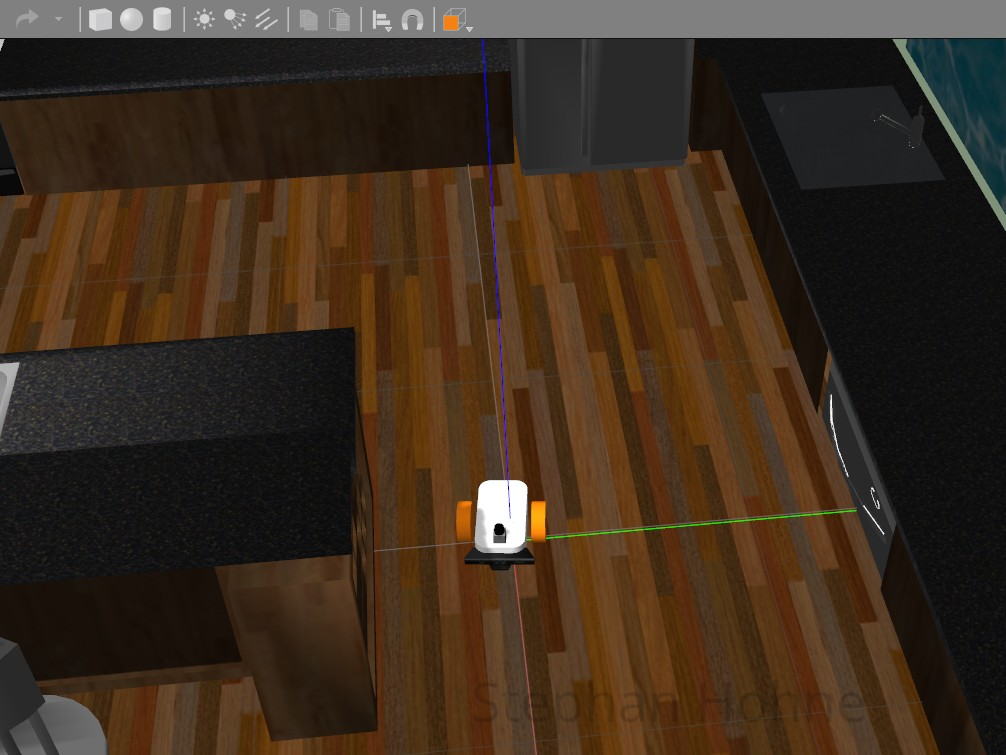
\includegraphics[width=\columnwidth]{images/kitchen_dining_rover_top.jpg}
      \caption{Rover model in the kitchen dining world viewed from the top. Screenshot taken in Gazebo.}
      \label{fig:rover_top}
\end{figure}

\begin{figure}[thpb]
      \centering
      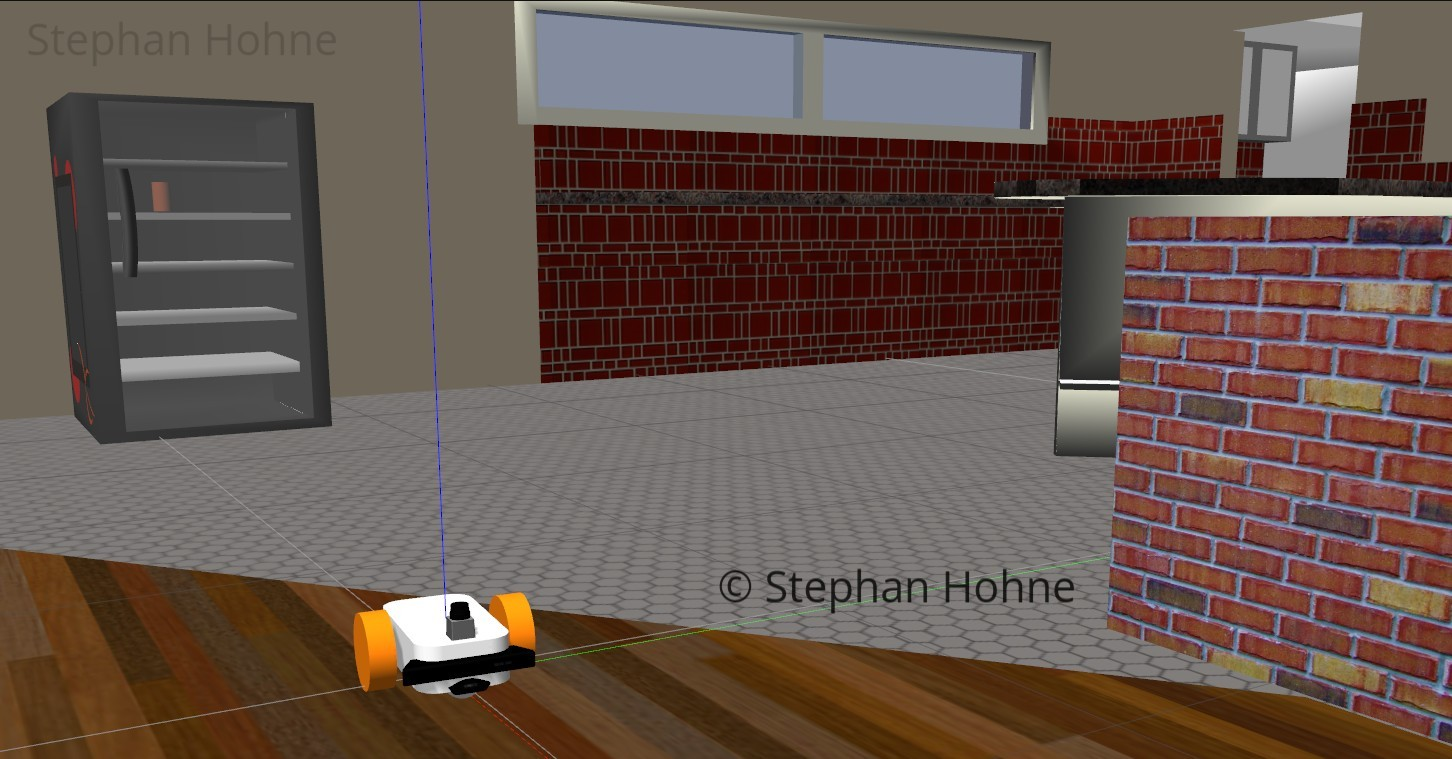
\includegraphics[width=\columnwidth]{images/rover_cafe_gazebo.jpg}
      \caption{View of the rover mapping the \texttt{cafe.world}. Screenshot taken in Gazebo.}
      \label{fig:cafe_world_gazebo_side}
\end{figure} 

\section{Background: Mapping}
\label{sec:background}
\subsection{Binary Bayes Filtering}
Occupancy grid mapping is a probabilistic method to generate a map with known locations of the robot. The robot and the environment are represented mathematically by a dynamical system. The robot path is given by the sequence of poses $x_{1:k}$ up to the current time step $k$, and the noisy measurements are represented by $y_k$. The goal is to implement an algorithm that determines the posterior probability distribution
\begin{equation}
\label{eqn:posterior_known_poses}
P\left( m \vert x_{1:k}, y_{1:k} \right) \, .
\end{equation}
The posterior is conditioned on the trajectory and all measurements up to the current time step.

The \ogm\ algorithm aims at determining the map $m$ that maximizes the posterior probability \ref{eqn:posterior_known_poses} using binary Bayes filtering. The 2D environment is uniformly partitioned into binary grid cells $m_l$ enumerated by the index $l = 1, \ldots, n$. Each cell stores the probability $P(m_l)$ of being occupied. The main assumption of occupancy grid mapping is that the cells can be considered independently so that the posterior turns into a product of marginals,
\begin{equation}
P\left( m \vert x_{1:k}, y_{1:k} \right)
=
\prod_{l=1}^{n}
P\left(m_l \vert x_{1:k},  y_{1:k}\right) \, .
\end{equation}
The remaining task is to find a posterior $P\left(m_l\vert x_{1:k},  y_{1:k}\right)$ for each of the $2^n$ cells and to describe how to update a single cell upon sensory input. The binary state of the map is static, it does not change during measurement, and the map states $m_l \in \left\lbrace 0,1\right\rbrace$ are much less complex than the measurements (for example a camera images). Therefore an inverse measurement model is applied to compute the belief $P\left(m_l \vert y_{1:k} \right)$. To represent the posterior belief mathematically, the log odds representation of probabilities is used. For the event $e$ with probability $p(e)$, the log odds representation is given by
\begin{equation}
\mathcal{O} \left(e\right) \coloneqq
\log 
\left(\frac{p\left(e\right)}{1-p\left(e\right)}\right) \, .
\end{equation}
The advantage of this representation is that factorized probabilities are turned into sums and numbers close to zero or one can be handled with better accuracy.

The binary Bayes filter algorithm computes the log odds of the posterior belief $l_k$ recursively according to
\begin{equation}
l_k = l_{k-1}
+ \mathcal{O} \left(m \vert y_k \right)
- \mathcal{O} \left(m \right) \, ,
\end{equation}
where $m$ is the binary state of the map and $y_k$ is the sensory input at step $k$. The second to last term represents the inverse measurement model and the last term represents the initial belief.

The occupancy grid algorithm assumes that the grid cells are independent of each other, that the measurements are independent, and that the environment has a binary structure, where cells can be either occupied or free. These assumptions reduce the original high-dimensional estimation problem into an independent set of one-dimensional problems, but they limit the range of applicability and the correctness of the resulting maps. In the real world, consecutive measurements and neighboring grid cells are typically correlated.

The maps generated by the algorithm can be visualized using RViz for 2D maps and the OctoMap software \cite{hornung13auro} for 3D maps. The occupancy grid mapping algorithm is used as a post-processing step for SLAM. It takes as input the poses filtered from SLAM and noisy measurements and generates a refined map that can be used for path planning and navigation.

\subsection{\gs}
\label{sec:graph_slam}
The \gs\ algorithm aims at solving the full SLAM problem \ref{eqn:posterior_full_slam}. The goal is to find the most likely robot path and map. The idea is to organize information in a graph. A node in the graph represents either a robot pose $x_t$ at a specific time step $t$ or the location of a feature in the environment denoted as $m^{\left(i\right)}$ with $i = 1. \ldots \alpha$. An edge in the graph represents either a measurement constraint between a pose and a feature or a motion constraint between two successive poses. Since the spatial constraint are soft, they can be considered as springs connecting two masses. In this analogy, the full SLAM problem can be solved as a global graph optimization problem. The optimal graph configuration is the one where the springs are relaxed, and the forces on each of the nodes are minimized. 

% The goal of \gs\ is to find the most likely robot path and map of the environment by creating a graph of all poses and features. The front-end of \gs\ constructs the graph from odometry and sensor inputs. It also must solve the data association problem, and detect loop closures. The back-end of \gs\ is responsible for graph optimization, it takes as input the complete graph with all constraints, and computes the most likely configuration of robot poses and map features, the system configuration that produces the smallest error.  

Formally, the maximum likelihood estimation (MLE) principle is applied to optimize the graph. The robot poses and map features are represented by random variables. The MLE technique tries to estimate the pose and map parameters that best explain the given measurements. Define a measurement update at time step $t$ as
\begin{equation}
\label{eqn:measurement_update}
\overline{z}_t \coloneqq  x_t + m_t^{\left(i\right)} \, ,
\end{equation}
which represents for instance a laser range finder measuring the distance to the landmark $m^{\left(i\right)}$. Equivalently, define a motion update as
\begin{equation}
\label{eqn:motion_update}
\overline{x}_t \coloneqq  x_{t-1} + u_t \, ,
\end{equation}
which could be realized as a control command instructing the robot to move a certain distance $u_t$. The update are assumed to have Gaussian noise. The corresponding probabilty distributions are given by 
\begin{eqnarray}
\label{eqn:gaussian_measurement_update}
p_m \left( z_t \right)  & = & 
\frac{1}{\sqrt{2 \pi} \sigma_m}
\exp \left(-\frac{1}{2}\left(\frac{z_t -\overline{z}_t}{\sigma_m}\right)^2 \right)
\\
\label{eqn:gaussian_motion_update}
p_u \left( x_t \right)  & = &
\frac{1}{\sqrt{2 \pi} \sigma_u}
\exp \left(-\frac{1}{2}\left(\frac{x_t -\overline{x}_t}{\sigma_u}\right)^2 \right)
\end{eqnarray}

In some simple cases it is possible to find an analytical solution to MLE by converting the target function to the negative log-likelihood form
\begin{equation*}
J_{\mathrm{\gs}} = \sum_t
\left(\frac{z_t - \overline{z}_t}{\sigma_{m}} \right)^2
+ \sum_t
\left(\frac{x_t - \overline{x}_t}{\sigma_{u}} \right)^2
\, ,
\end{equation*}
trying to minimize the sum of all constraints. In more complex realistic scenarios, approximate numerical solutions are needed, for instance by applying gradient descent techniques.

States and measurements in the real world are multi-dimensional, and must be expressed as vectors $\mathbf{x}_t$ and $\mathbf{z}_t$, respectively. The constraints are given by
\begin{eqnarray}
\mathbf{v}_t & \coloneqq &
\mathbf{z}_t - h \left(\mathbf{x}_t , m_t \right) \, ,  
\\
\mathbf{w}_t & \coloneqq &
\mathbf{x}_t - g \left(\mathbf{x}_{t-1} , u_t \right) \, ,
\end{eqnarray}
where $h$ is the measurement model and $g$ is the motion model. Noise is represented by covariance matrices $Q$ for the sensor model and $R$ for the motion model. The estimation function is given by
\begin{equation*}
J_{\mathrm{\gs}} =
\mathbf{x}_{0}^{\mathrm{T}} \Omega_{0} \mathbf{x}_{0}
+ \sum_t \left(
\mathbf{w}_{t}^{\mathrm{T}} R_{t}^{-1} \mathbf{w}_{t} +
\mathbf{v}_{t}^{\mathrm{T}} Q_{t}^{-1} \mathbf{v}_{t}
\right) \, .
\end{equation*}

To store constraint information efficiently, the information matrix $\Omega$ and the information vector
\begin{equation*}
\xi = \left( x_0 , \ldots , x_t , m_1 , \ldots , m_{\alpha} \right)
\end{equation*}
are introduced. The information matrix is inverse to the covariance. Once all the information is collected, the path and map are inferred from the information matrix and vector by the inversion operation $\Omega^{-1} \xi$. The resulting vector contains the best guess estimate for all poses and features.

The \gs\ algorithm solves the full SLAM problem. It has an improved accuracy over FastSLAM and reduces the need for on-board processing. Since it recovers the full path of the robot and the entire map, it can detect correlations between current and previous poses.

\rtab\ is a graph based SLAM approach that uses image data collected from vision sensors like a RGB-D camera to localize the robot, map the environment, and detect loop closures \cite{labbe14online, labbe13appearance}. Image features are compared in order to determine if the robot has seen a location before. During a mapping run, the number of images to be processed increases linearly, and so does the complexity of the loop closure algorithm. \rtab\ is optimized for long-term mapping and can do loop closure in real time. In contrast to the landmark based constraints discussed above, \rtab\ considers only odometry constraints and loop closure constraints. \rtab\ is able to generate 2D and 3D occupancy grid maps as well as 3D point clouds.

\section{Model Configuration}
\label{sec:model_configuration}
The ROS package \href{https://github.com/S2H-Mobile/RoboND-SLAM-Project/tree/master/slam_rover}{\texttt{slam\_rover}} defines two Gazebo worlds and a rover model that employs the \rtab\ package to perform SLAM of both environments. For ease of reuse of the components, the package is organized in folders containing the robot model URDF files, Gazebo SDF files, meshes, scripts, configuration files and launch files.

\begin{figure*}[thpb]
      \centering
      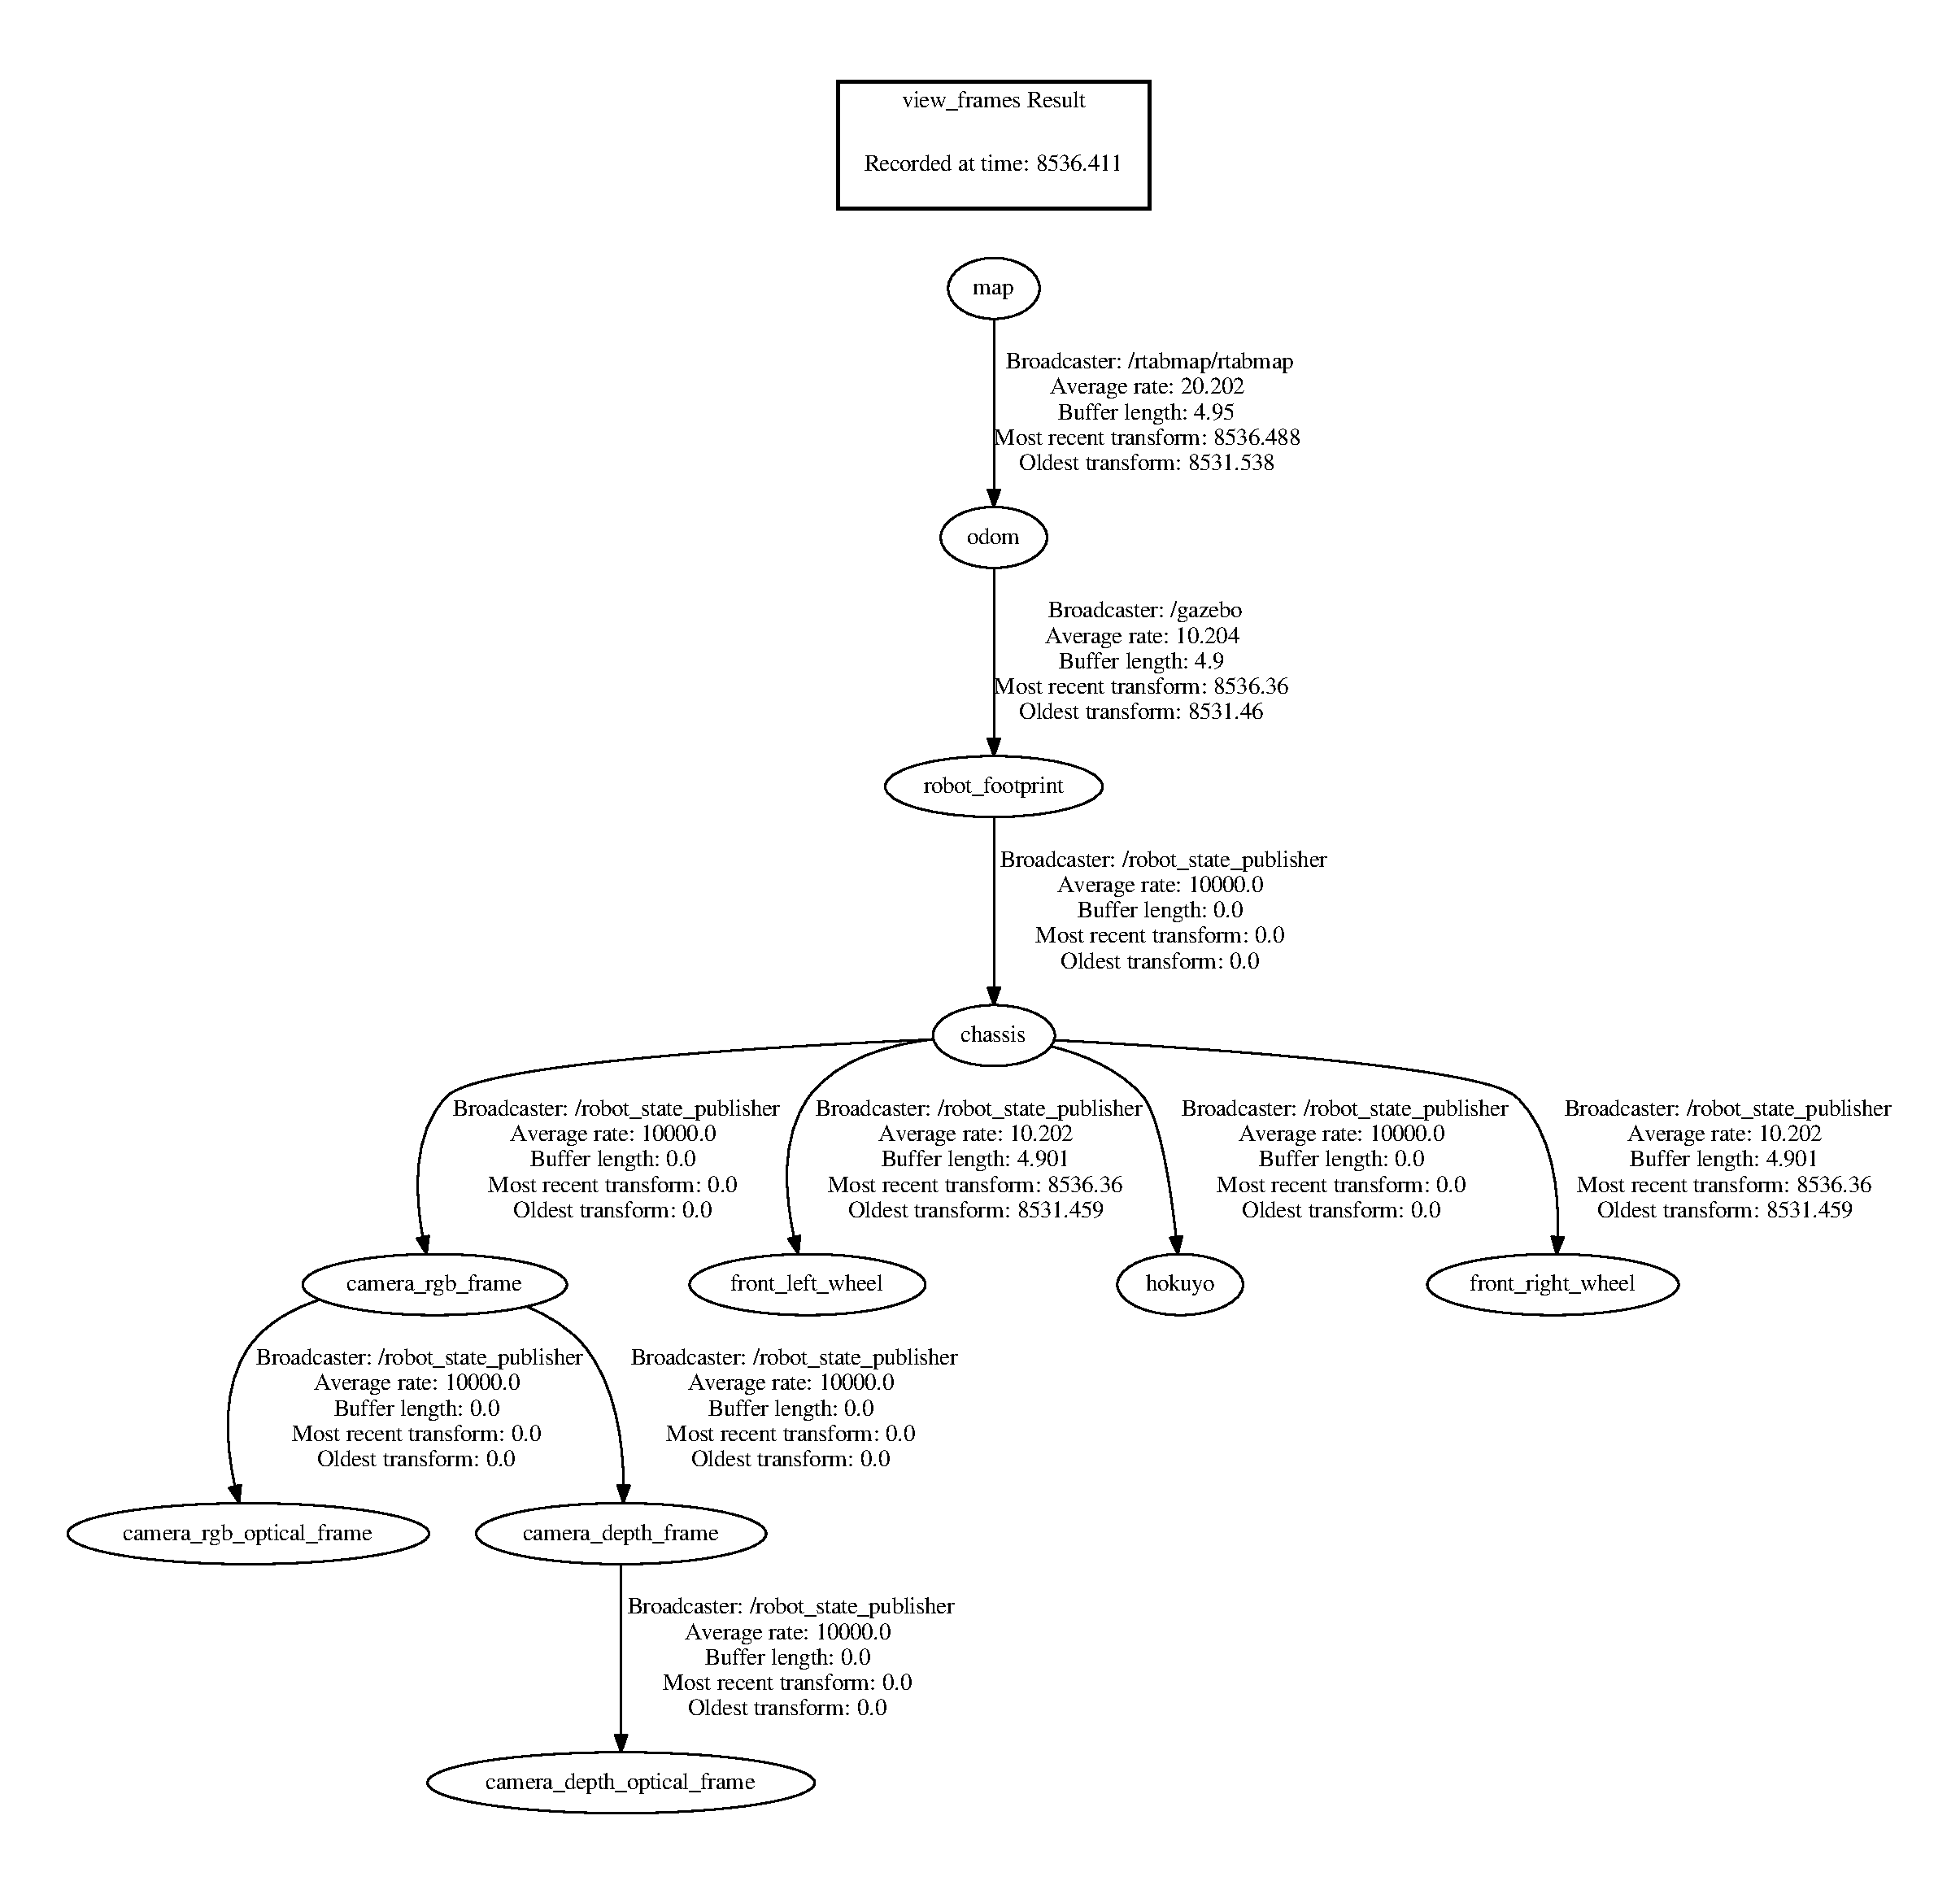
\includegraphics[width=\textwidth]{images/frames.pdf}
      \caption{Transform tree of the rover model. Output from \texttt{rosrun tf2\_tools view\_frames.py}.}
      \label{fig:rover_tf_tree}
\end{figure*}

The \texttt{urdf} folder contains the file \texttt{rover.xacro} defining the links and joints of the robot model used for physics simulation and visualization as well as the file \texttt{rover.gazebo} specifying the Gazebo plugins for differential drive, RGB-D camera and laser range finder. See section \ref{sec:robot_model} for details. Besides the environments provided as student material, the \texttt{worlds} directory includes the file \texttt{cafe.world} defining a custom indoor environment in SDF markup, see section \ref{sec:world_creation} for details. The image and mesh files necessary to model the Hokuyo laser and Kinect camera are downloaded from the \href{https://bitbucket.org/osrf/gazebo_models/downloads/}{Gazebo model database} and stored in the \texttt{meshes} folder. The \texttt{launch} folder contains four ROS node launch configurations, as detailed in section  \ref{sec:ros_launch}. The \texttt{config} directory contains the RViz configuration file, and a script for tele-operating the rover can be found in \texttt{scripts}. 

\subsection{Robot Model}
\label{sec:robot_model}
The rover model is shown in figures \ref{fig:rover_top} and \ref{fig:cafe_world_gazebo_side}. The URDF specification can be found in \href{https://github.com/S2H-Mobile/RoboND-SLAM-Project/blob/master/slam_rover/urdf/rover.xacro}{\texttt{rover.xacro}}. The transform tree associated to the robot geometry is shown in figure \ref{fig:rover_tf_tree}.

To create the robot model, the mobile rover from \cite{where_am_i} is taken as a starting point. The chassis is left as in the original model, with two parallel wheels at the sides. The wheels are driven differentially. Caster wheels in the front and back stabilize the body while allowing the robot to rotate in place. To enable the robot to perform appearance based mapping using visual odometry, the generic RGB camera of the original model is upgraded to a Kinect RGB-D camera. The camera is mounted to the front of the chassis to allow for unobstructed view, facing in forward direction. The mesh files for the \href{http://models.gazebosim.org/kinect/}{Kinect camera} model are downloaded from the \href{https://bitbucket.org/osrf/gazebo_models/downloads/}{Gazebo model database} and included in the \texttt{slam\_rover/meshes} folder.  Like the original model, the rover is fitted with a Hokuyo 2D laser range finder. The corresponding \texttt{hokuyo} link is mounted with a fixed joint on the top of the chassis, to let the laser beans rotate without hitting any part of the robot.
the laser range finder provides more precise localization and thereby refines geometric constraints

The differential drive plugin is configured in the \texttt{rover.gazebo} file to publish control commands to the \texttt{/cmd\_vel} topic and odometry messages to the \texttt{/odom} topic. The camera plugin is configured to publish raw RGB images to \texttt{/camera/rgb/image\_raw} and raw depth images to \texttt{/camera/depth/image\_raw}. The laser plugin is configured to publish messages of type \texttt{LaserScan} to the \texttt{/slam\_rover/laser/scan} topic. A graphical view of the ROS topics and nodes is shown in figure \ref{fig:rqt_graph}.

\begin{figure*}[thpb]
      \centering
      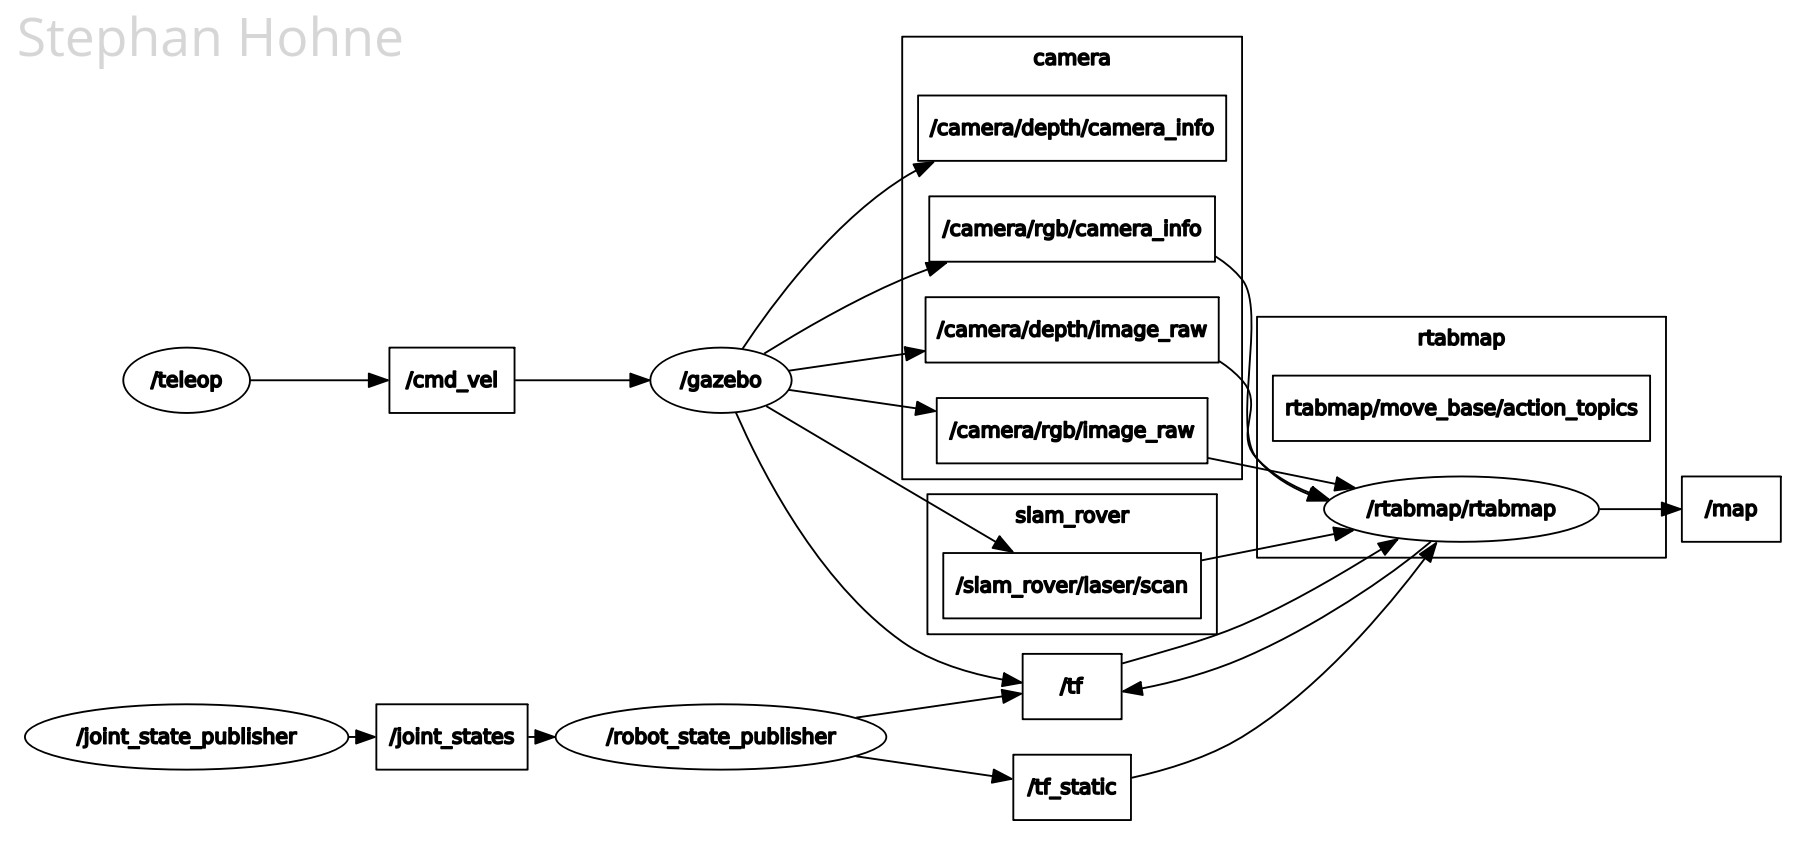
\includegraphics[width=\textwidth]{images/rqt_graph.jpg}
      \caption{Active topics when all nodes are launched. Output from \texttt{rqt\_graph}.}
      \label{fig:rqt_graph}
\end{figure*}

\subsection{World Creation}
\label{sec:world_creation}
As part of the project, the custom \texttt{cafe.world} is created in Gazebo. This indoor environment is based on the \href {http://models.gazebosim.org/cafe/}{cafe model} from the Gazebo database. The base model consists of a large room with a bar reaching into the room, and a separate kitchen. The kitchen can not be entered by the robot. Several items are added to the base model to serve as distinctive elements in the environment, such as tables, a ladder, a fountain, and a block made of red bricks. The large room is separated in two parts of approximately equal size by a white wall oriented in $x$-direction. A bird's eye view of the cafe world which also serves as the ground truth for mapping is shown in figure \ref{fig:cafe_world_gazebo_top}. An image of the rover navigating the cafe world is shown in figure \ref{fig:cafe_world_gazebo_side}.

\begin{figure}[thpb]
      \centering
      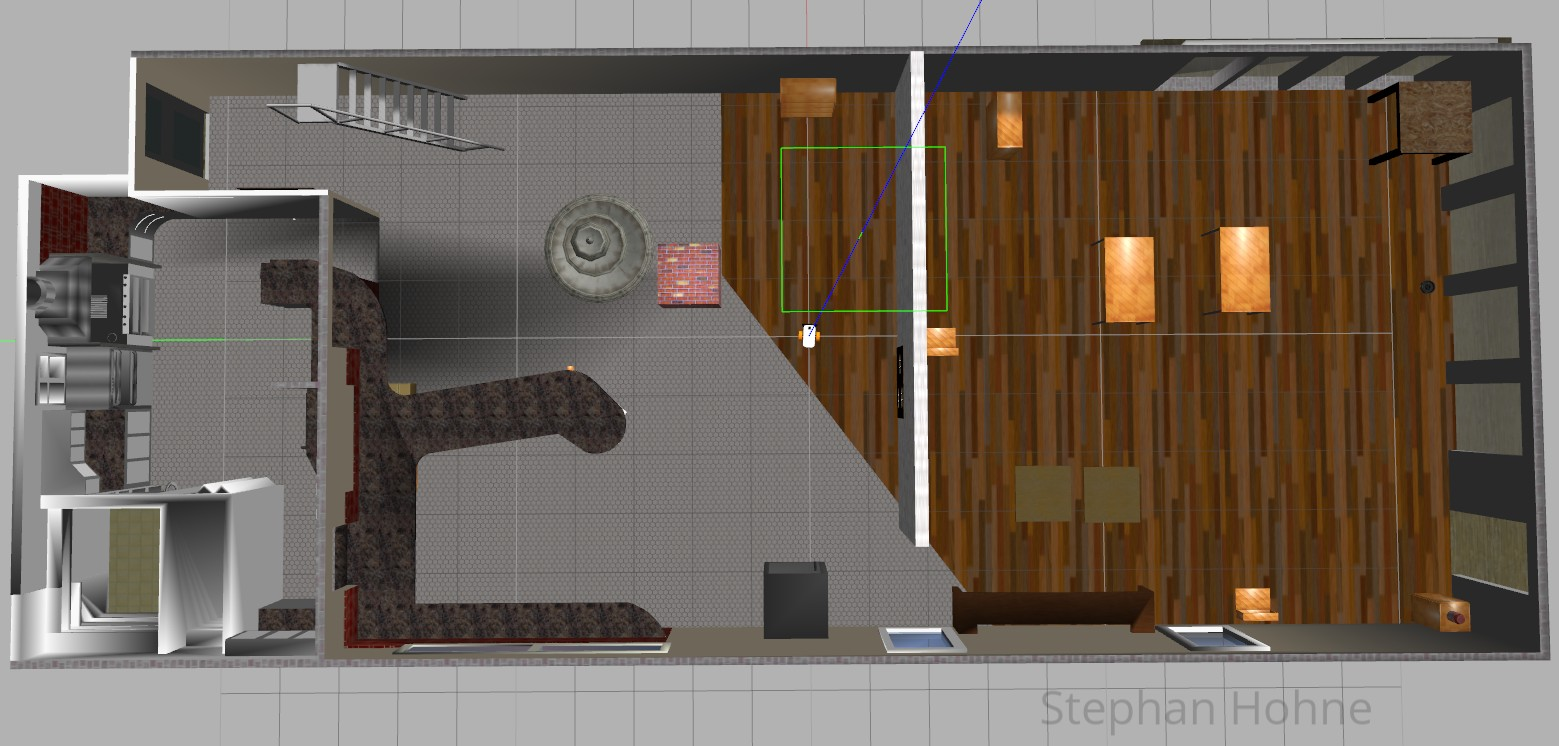
\includegraphics[width=\columnwidth]{images/cafe_world_gazebo.jpg}
      \caption{View of the rover in the \texttt{cafe.world} from above. Screenshot taken in Gazebo.}
      \label{fig:cafe_world_gazebo_top}
\end{figure}

\subsection{ROS Launch Configuration}
\label{sec:ros_launch}
Four ROS nodes need to be launched in order to let the robot perform a mapping run in one of the environments. The \texttt{world.launch} file starts the Gazebo physics simulation of the rover in one of the environments. The world file, which can be either \texttt{kitchen\_dining.world} or \texttt{cafe.world}, is specified inside the launch file. The \rtab\ node is started with the \href{https://github.com/S2H-Mobile/RoboND-SLAM-Project/blob/master/slam_rover/launch/mapping.launch}{\texttt{mapping.launch}} file. The node is configured for visual loop closures using the SURF detection method. A minimum of $15$ visual features must coincide for loop closure to be accepted. The \texttt{rviz.launch} file starts visualization of the rover, sensor data, as well as map and camera topics in RViz. See images \ref{fig:rover_kitchen_dining_rviz} and \ref{fig:rover_cafe_rviz} for screenshots taken during mapping of each world. The \texttt{teleop.launch} file starts the teleoperation script provided as student material. The script lets the user remote control the robot model. 
\begin{figure}[thpb]
      \centering
      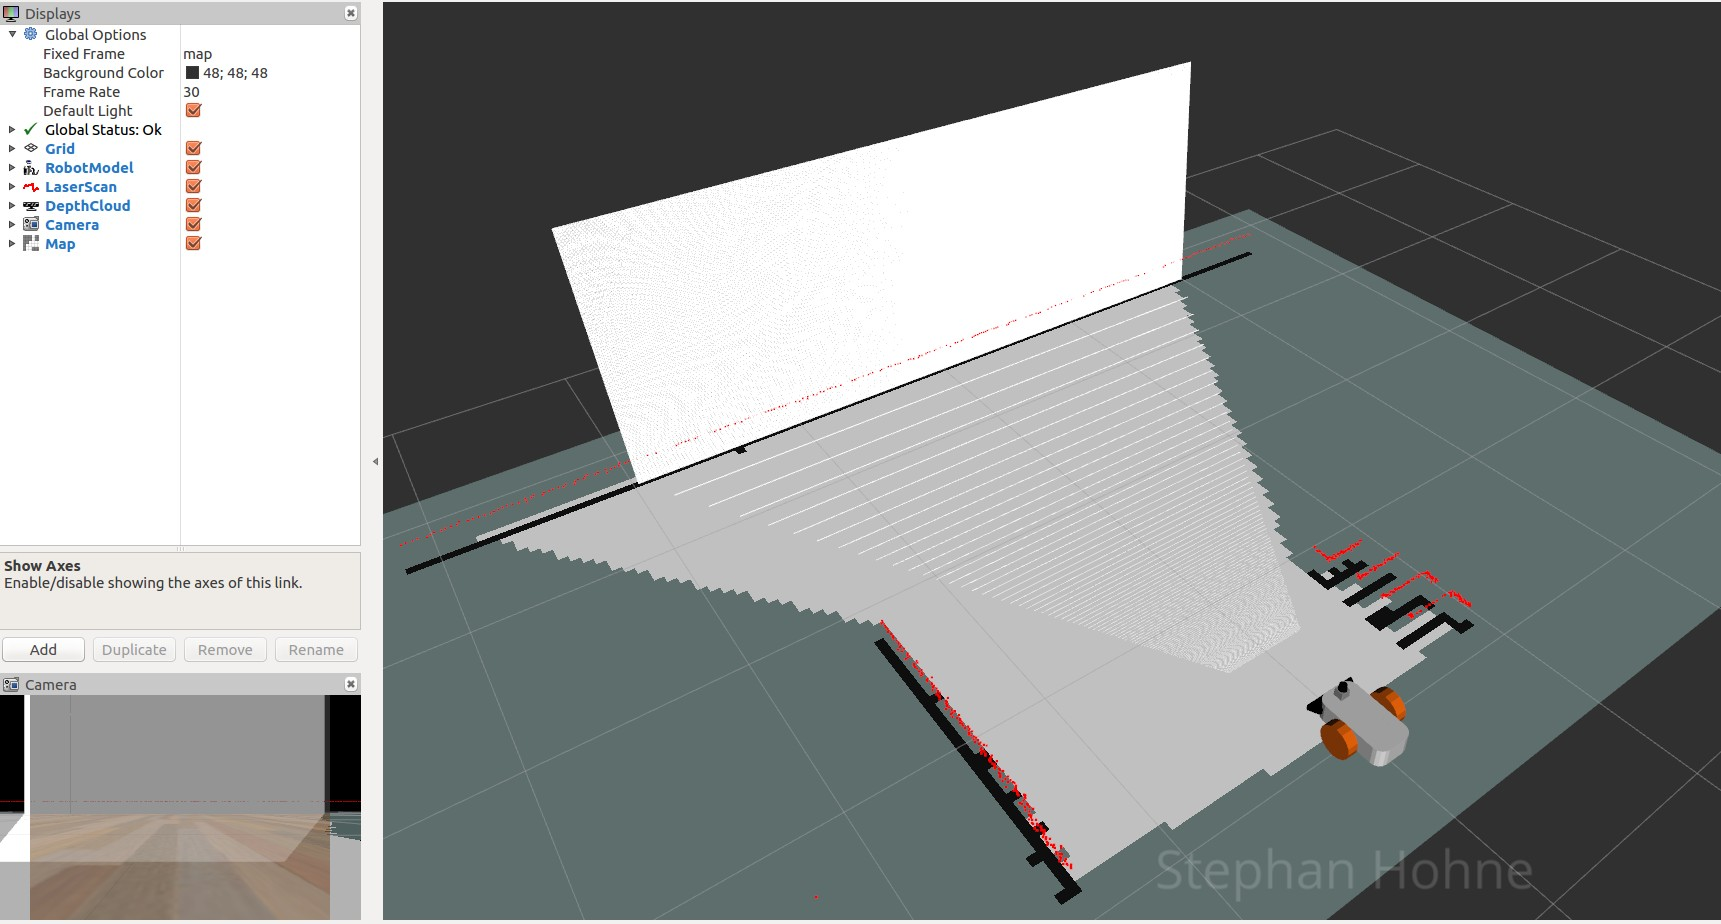
\includegraphics[width=\columnwidth]{images/rover_kitchen_dining_rviz.jpg}
      \caption{View of the rover mapping the \texttt{kitchen\_dining.world}. Screenshot taken in RViz.}
      \label{fig:rover_kitchen_dining_rviz}
\end{figure}
\begin{figure}[thpb]
      \centering
      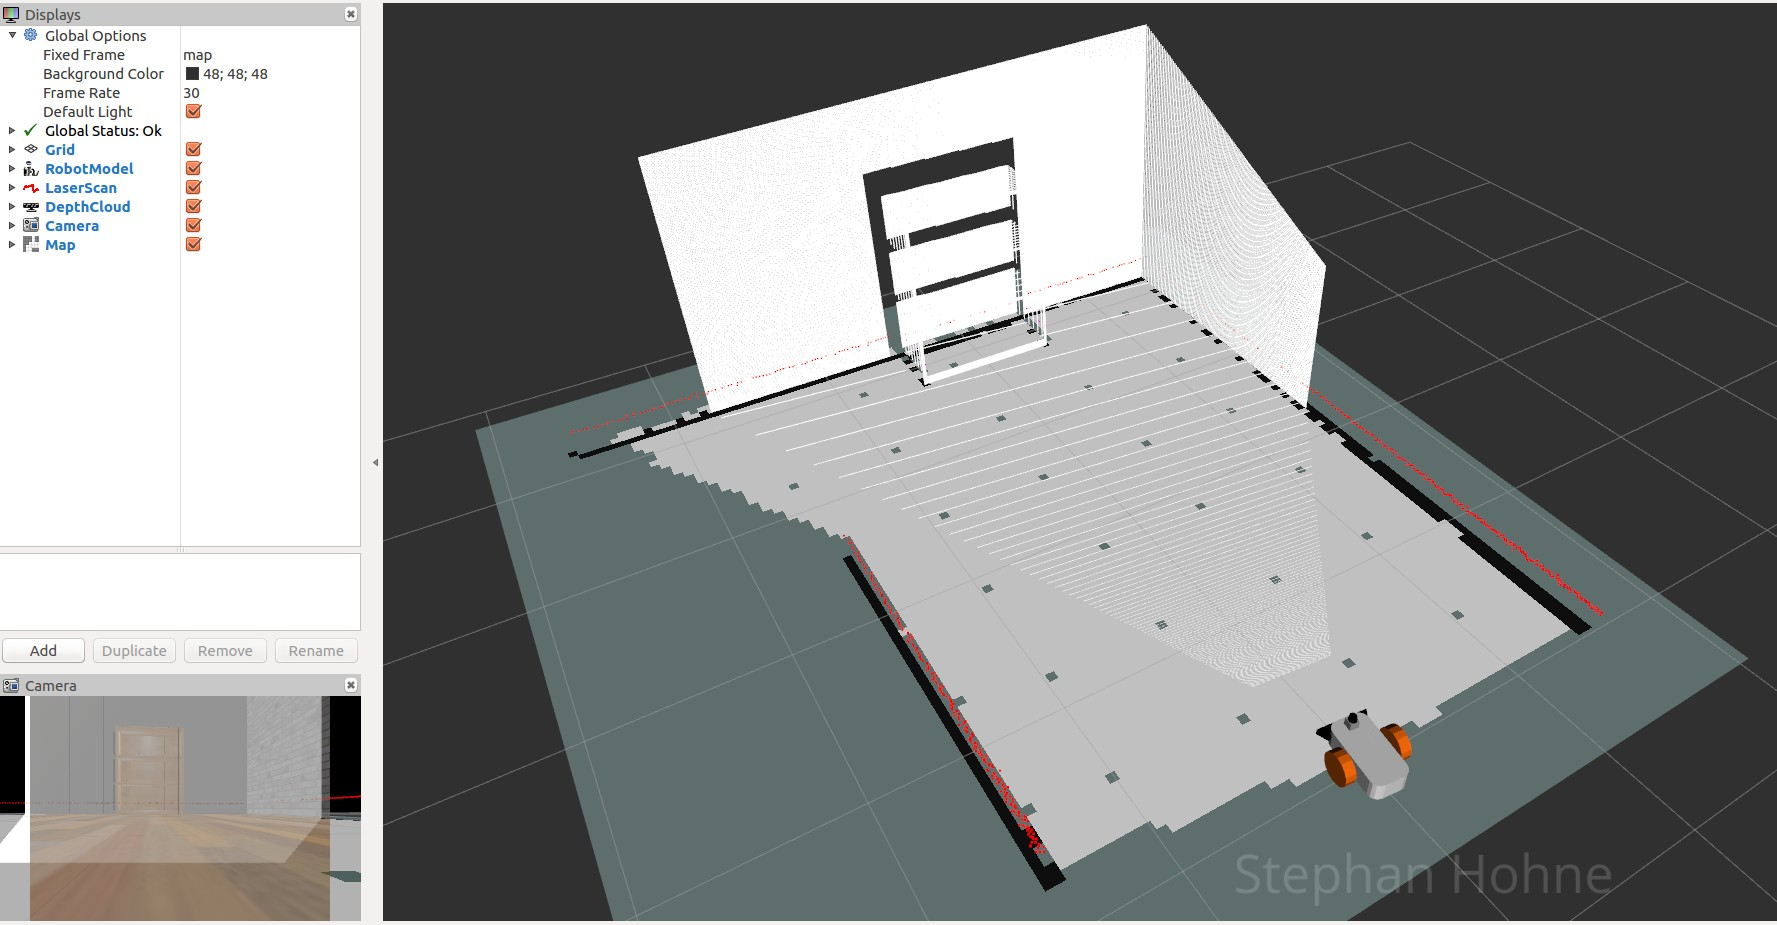
\includegraphics[width=\columnwidth]{images/rover_cafe_rviz.jpg}
      \caption{View of the rover mapping the \texttt{cafe.world}. Screenshot taken in RViz.}
      \label{fig:rover_cafe_rviz}
\end{figure}

When all the four aforementioned nodes are launched, the robot is able to perform mapping of the given environment. During the mapping run, the map data are stored in the \texttt{rtabmap.db} database. The full set of active topics and nodes during a mapping run is shown in figure \ref{fig:rqt_graph}. The \texttt{localization.launch} file can be started in order to localize the robot during the run.  

\section{Results}
\label{sec:results}
Remote controlled mapping runs were performed in both worlds. In order to collect enough images for comparison, the rover was steered $2$ or $3$ times across each room in each environment. During the runs, visualization of the generated 2D occupancy grid maps was achieved using RViz, as shown in figures \ref{fig:rover_kitchen_dining_rviz} and \ref{fig:rover_cafe_rviz}. When the mapping runs were finished, the resulting map databases were evaluated using the \rtab\ Database Viewer.
\subsection{Kitchen Dining World}
Mapping run $1$ in the kitchen dining world resulted in a graph with $140$ global loop closures. The \rtab\ database created during this mapping run can be downloaded as a \href{https://drive.google.com/open?id=1t1IpTFzVJdJpQvhg2gkvDuGDFBH2YYIq}{shared file} (approx.\ 155 MB download, file name is \texttt{rtabmap\_kitchen\_dining\_run1.db}).

The database was evaluated using \rtab \ Database Viewer. Instances of loop closures were examined and visualized, see figures \ref{fig:loop_closure_1}, \ref{fig:loop_closure_2}, \ref{fig:loop_closure_3}, \ref{fig:loop_closure_4}. Yellow circles indicate image features, and pink circles indicate image features that match different points on the robot trajectory.

The robot trajectory while traversing the kitchen dining world and the graph view of the resulting 2D occupancy grid are shown in figure \ref{fig:graph_view_kitchen_dining_small}. The 2D map overlaid on the occupancy grid is shown in figure \ref{fig:occupancy_grid_kitchen_dining}. 

\begin{figure}[thpb]
      \centering
      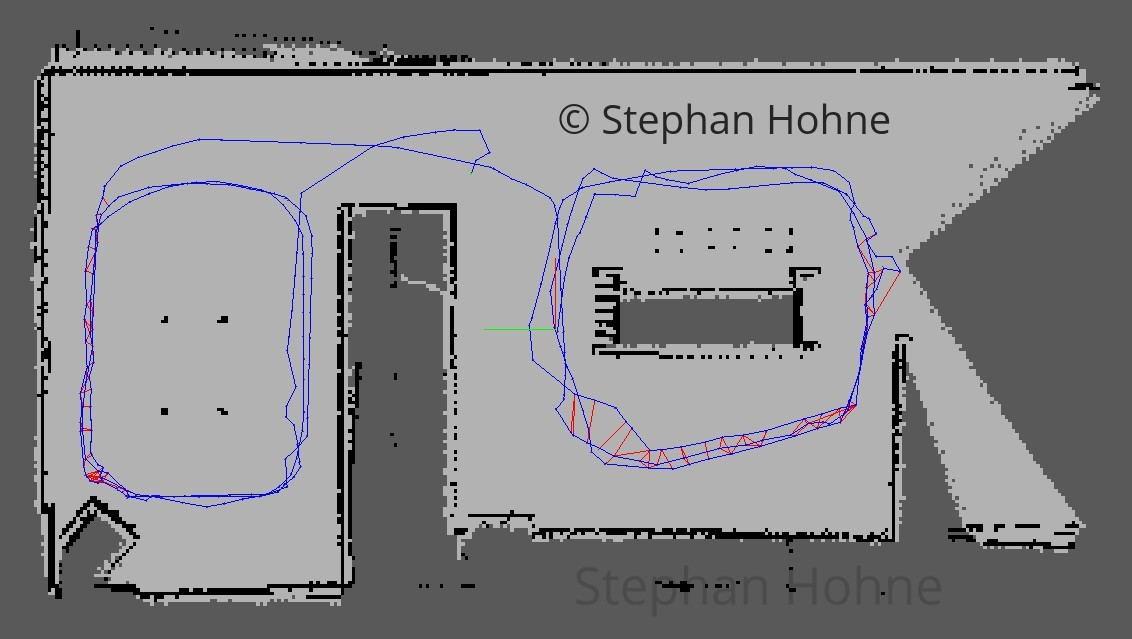
\includegraphics[width=\columnwidth]{images/graph_view_kitchen_dining_small.jpg}
      \caption{Robot path and 2D map of kitchen dining world created during mapping run $1$. Screenshot taken in \rtab\ Database Viewer.}
      \label{fig:graph_view_kitchen_dining_small}
\end{figure}

\begin{figure}[thpb]
      \centering
      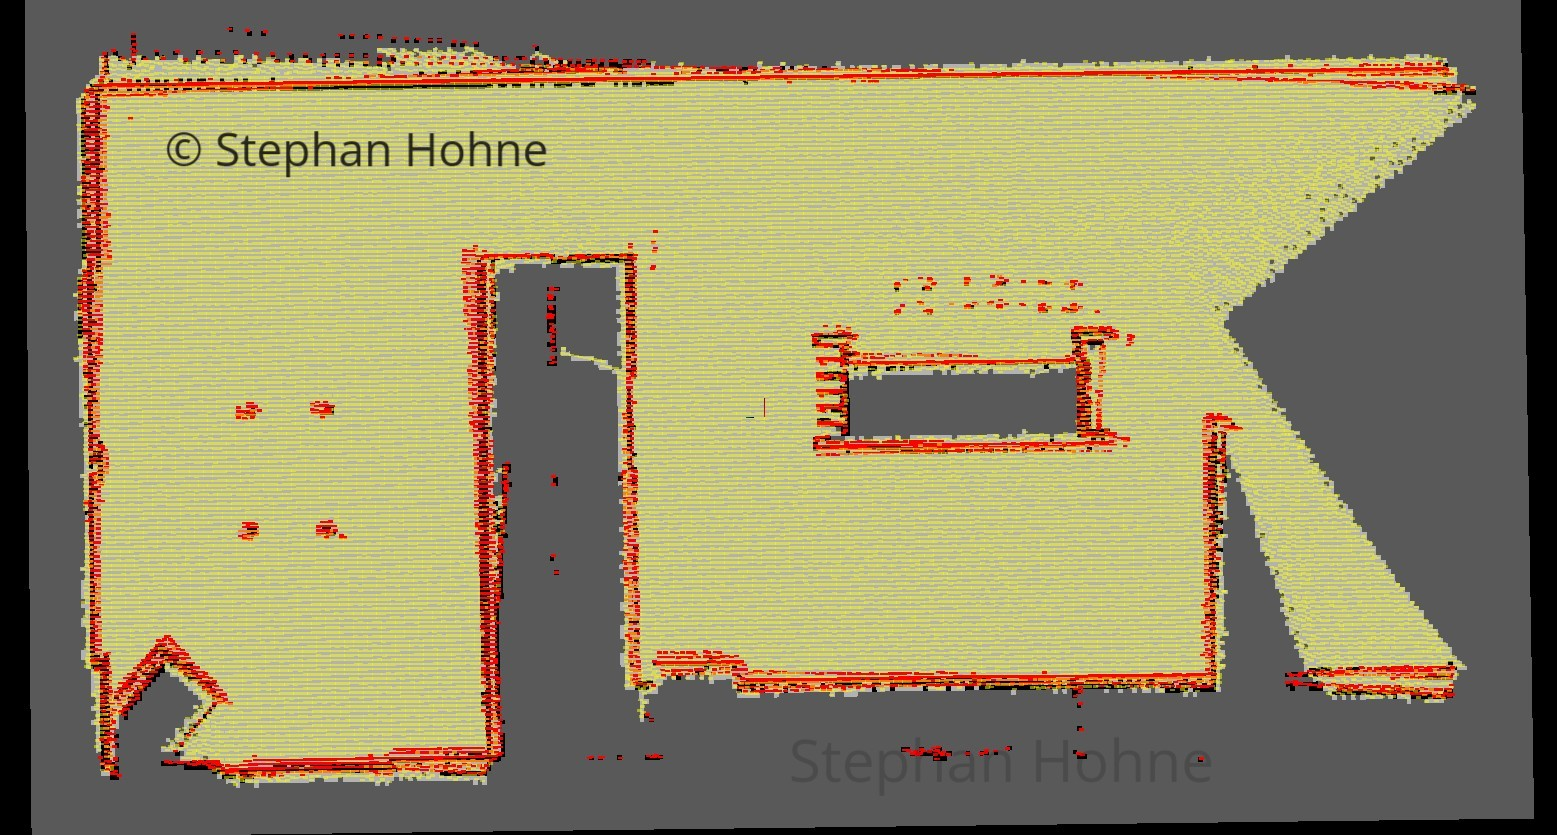
\includegraphics[width=\columnwidth]{images/occupancy_grid_kitchen_dining.jpg}
      \caption{2D map and occupancy grid of kitchen dining world created during mapping run $1$. Screenshot taken in \rtab\ Database Viewer.}
      \label{fig:occupancy_grid_kitchen_dining}
\end{figure}

The \emph{Export 3D Clouds} functionality was then used to reconstruct 3D point clouds. In the first export, the default settings were kept. Figure \ref{fig:3d_point_cloud_kitchen_dining_default} shows the resulting reconstruction of the kitchen dining world. The features in the environment like tables and chairs are recognizable, see the further discussion in section \ref{sec:discussion}.

In the second export, all available algorithms for enhancement of the reconstruction were enabled. The options are cloud filtering, cloud smoothing, gain compensation, and meshing. The full export configuration can be downloaded as a \href{https://drive.google.com/open?id=1bmjYFEaccEG5NGRl02-8-JeOp9Mh6Myq}{shared file}. The resulting 3D point cloud of the kitchen dining world is shown in figure \ref{fig:3d_point_cloud_kitchen_dining_enhanced}, for a discussion see section \ref{sec:discussion}.

\subsection{Cafe World}
Mapping run $2$ in the cafe world resulted in a graph with $90$ global loop closures. The \rtab\ database created during this mapping run can be downloaded as a \href{https://drive.google.com/file/d/1fHX3h5c7w3LujcECYeHjkJM_bD-jZVOq/view?usp=sharing}{shared file} (approx.\ 105 MB download, file name is \texttt{
rtabmap\_cafe\_run2.db}). The resulting database was again evaluated in \rtab\ database  viewer. A 2D map and occupancy grid of the cafe world is shown in figure \ref{fig:rtabmap_occupancy_grid_cafe}.
\begin{figure}[htbp]
      \centering
      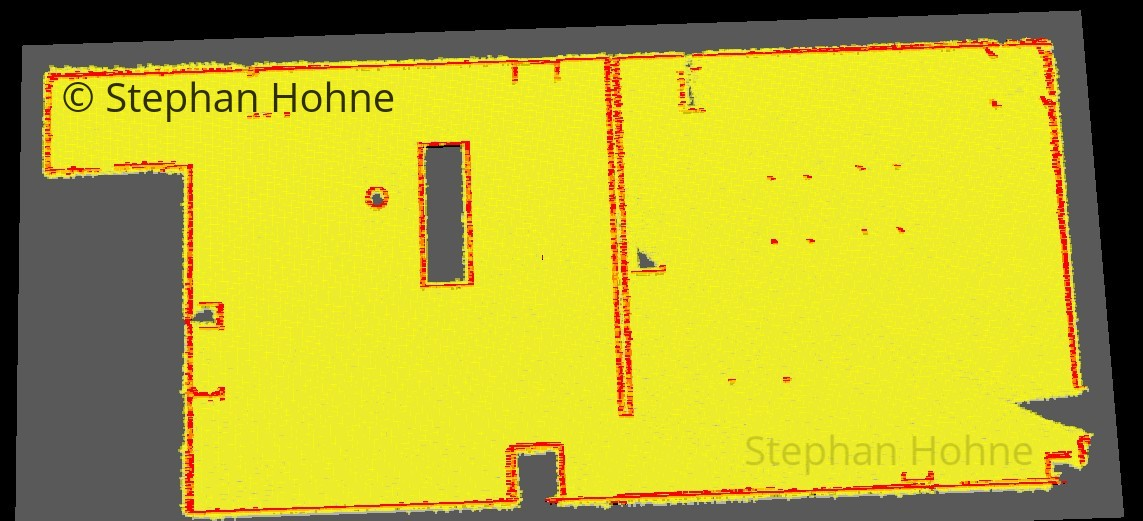
\includegraphics[width=\columnwidth]{images/rtabmap_occupancy_grid_cafe.jpg}
      \caption{2D map and occupancy grid of cafe world created during mapping run $2$. Screenshot taken in \rtab\ Database Viewer.}
      \label{fig:rtabmap_occupancy_grid_cafe}
\end{figure}

The robot path traversing the cafe world is shown in figure \ref{fig:graph_view_cafe} below. For this run, $90$ global loop closures were detected. An example loop closure between index $43$ and $55$ is shown in figure \ref{fig:loop_closure_cafe}. The \rtab\ tool was used to export 3D reconstructions as before. Figure \ref{fig:cafe_3D_default} shows the exported 3D point cloud using the default settings. Characteristic features of the environment like the ladder, tables and brick column are recognizable, see further discussion in section \ref{sec:discussion}. More exports were done with enhanced reconstruction settings, equal to those for the kitchen dining world. The resulting 3D views of the cafe world are shown in figures \ref{fig:cafe_3D_left} and \ref{fig:cafe_3D_right}.

\section{Discussion}
\label{sec:discussion}
The overall goal of generating 2D occupancy grid maps and 3D visualizations of both the \texttt{kitchen\_dining.world} and the custom \texttt{cafe.world} has been achieved. The generated 2D and 3D maps contain characteristic features, so that the ground truth environments can be recognized. 

There were instances of apparent mapping errors, where the spatial relationships of elements could not be reproduced correctly. The most notable example is the chair in the lower left corner of the dining room in the kitchen dining world, see image \ref{fig:3d_point_cloud_kitchen_dining_default} and \ref{fig:3d_point_cloud_kitchen_dining_enhanced}. In the reconstruction, the chair seems to be rotated by $\pi/2$ around the $z$-axis when compared to the ground truth world.

In the cafe world, the robot sensors did not recognize the bar reaching into the left room. Therefore this feature is missing in the map, see for instance figure \ref{fig:rtabmap_occupancy_grid_cafe}. The most probable explanation is that the walls of the bar are made of glass and therefore transparent. The footprint of the brick column is quadratic in Gazebo, see image \ref{fig:cafe_world_gazebo_top}, but rectangular in the 2D map, see image \ref{fig:rtabmap_occupancy_grid_cafe}.

The generated 2D and 3D maps can be improved in quality and detail by doing mapping runs that cover the environment completely, and by further inspecting and optimizing the loop closures detected by \rtab .

\section{Future Work}
\label{sec:future_work}
It is desirable to explore more of the visualization options of the \rtab\ software. For instance, it will be interesting to create 3D occupancy grid maps by enabling the \texttt{Grid/3D} and \texttt{Grid/FromDepth} parameters in the \rtab\ ROS package. Another interesting 3D visualization option is to install the \href{https://octomap.github.io/}{Octomap} package.

A physical mobile robot based on the Jetson TX2 is under construction. The plan is to deploy the mapping stack developed here to it. A reasonable first task for \rtab\ is to create a map of the Wifi coverage of the environment, following the \href{http://wiki.ros.org/rtabmap_ros/Tutorials/WifiSignalStrengthMappingUserDataUsage}{ROS Wiki tutorial}. 

\begin{figure*}[thpb]
      \centering
      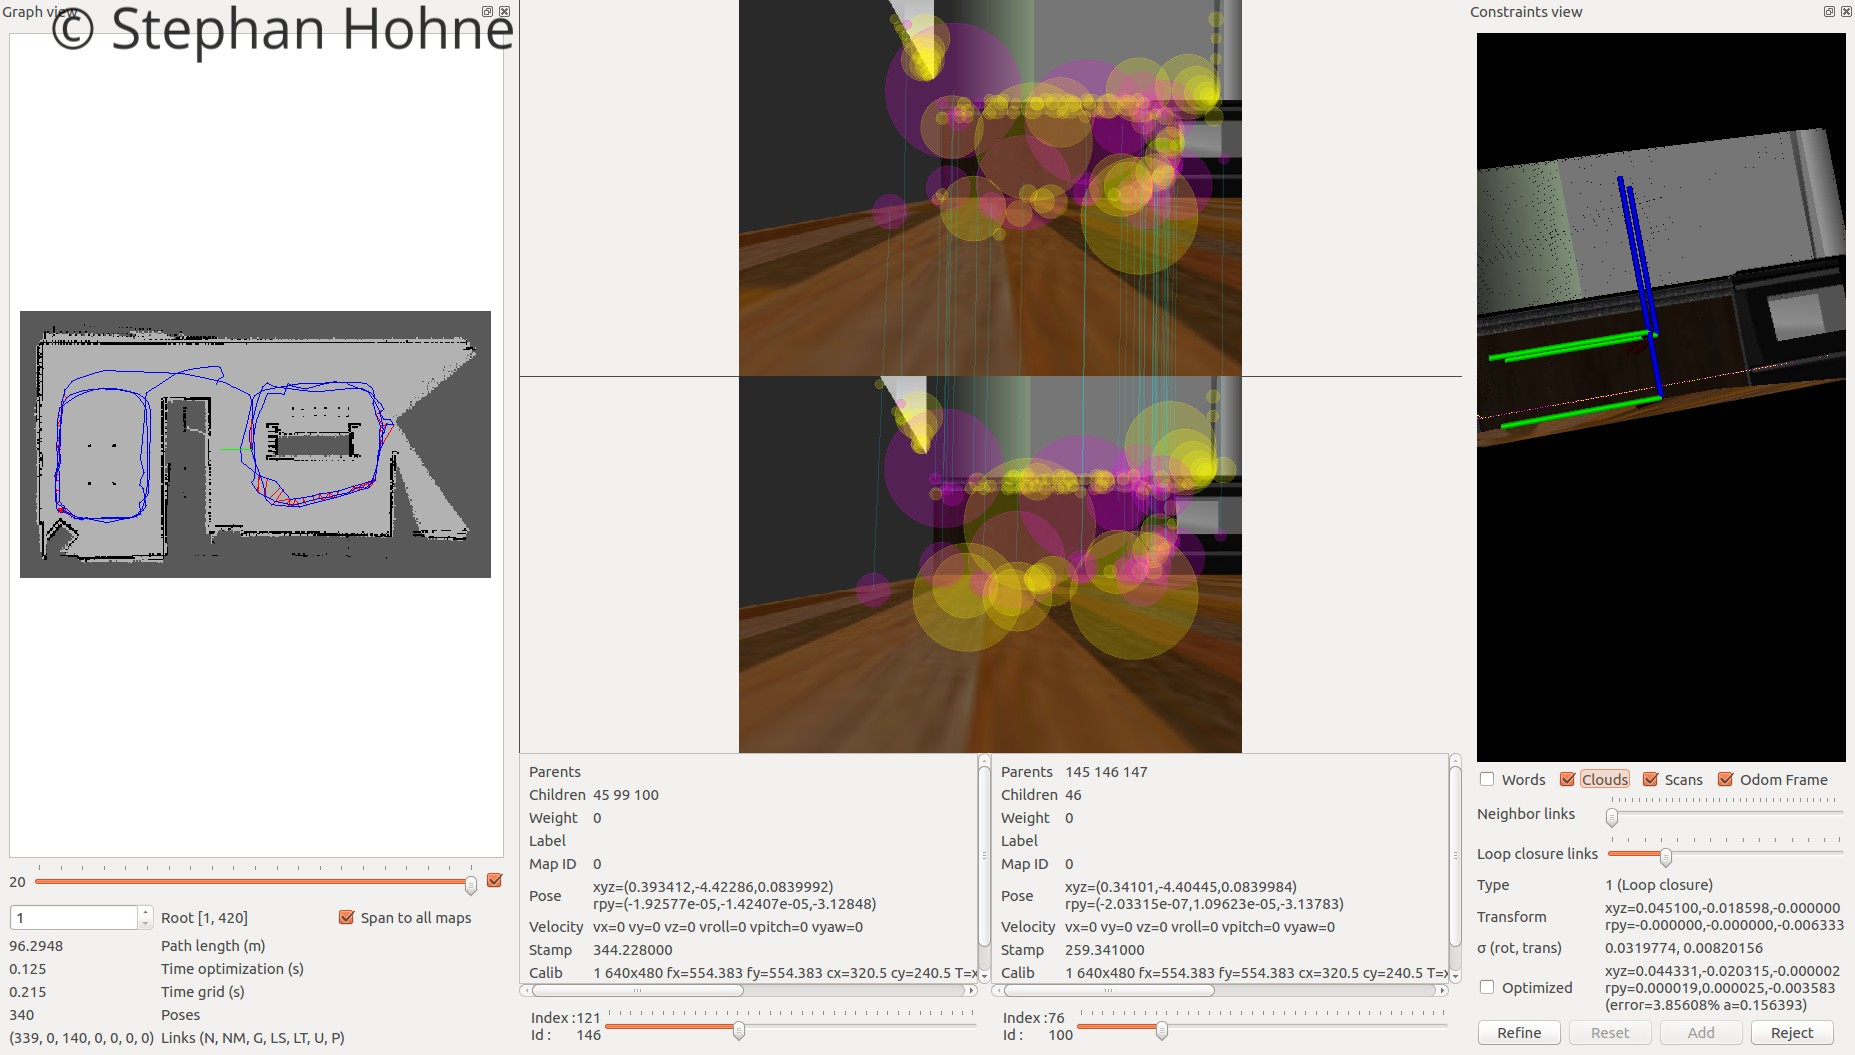
\includegraphics[width=\textwidth]{images/loop_closure_1.jpg}
      \caption{Loop closure in the map database \texttt{rtabmap\_kitchen\_dining\_run1.db}. Screenshot taken in \rtab\ Database Viewer.}
      \label{fig:loop_closure_1}
\end{figure*}

\begin{figure*}[thpb]
      \centering
      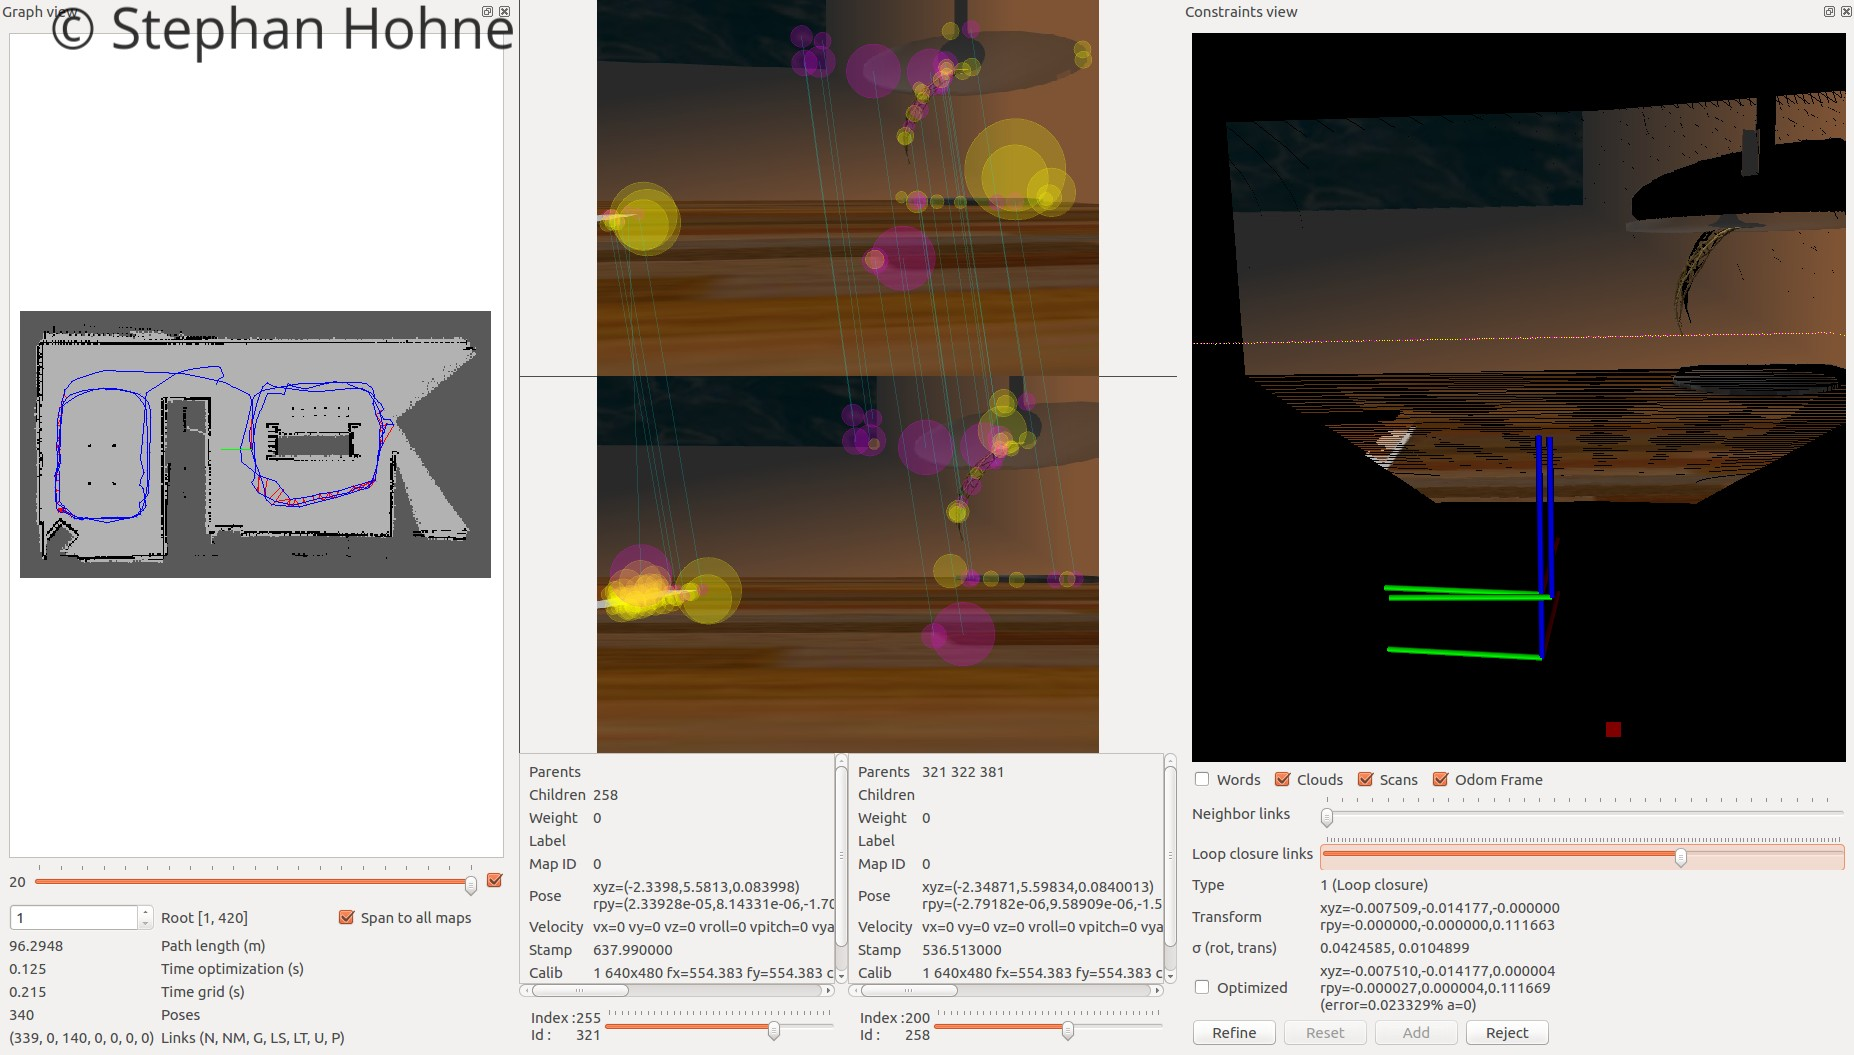
\includegraphics[width=\textwidth]{images/loop_closure_2.jpg}
      \caption{Loop closure in the map database \texttt{rtabmap\_kitchen\_dining\_run1.db}. Screenshot taken in \rtab\ Database Viewer.}
      \label{fig:loop_closure_2}
\end{figure*}
\begin{figure*}[thpb]
      \centering
      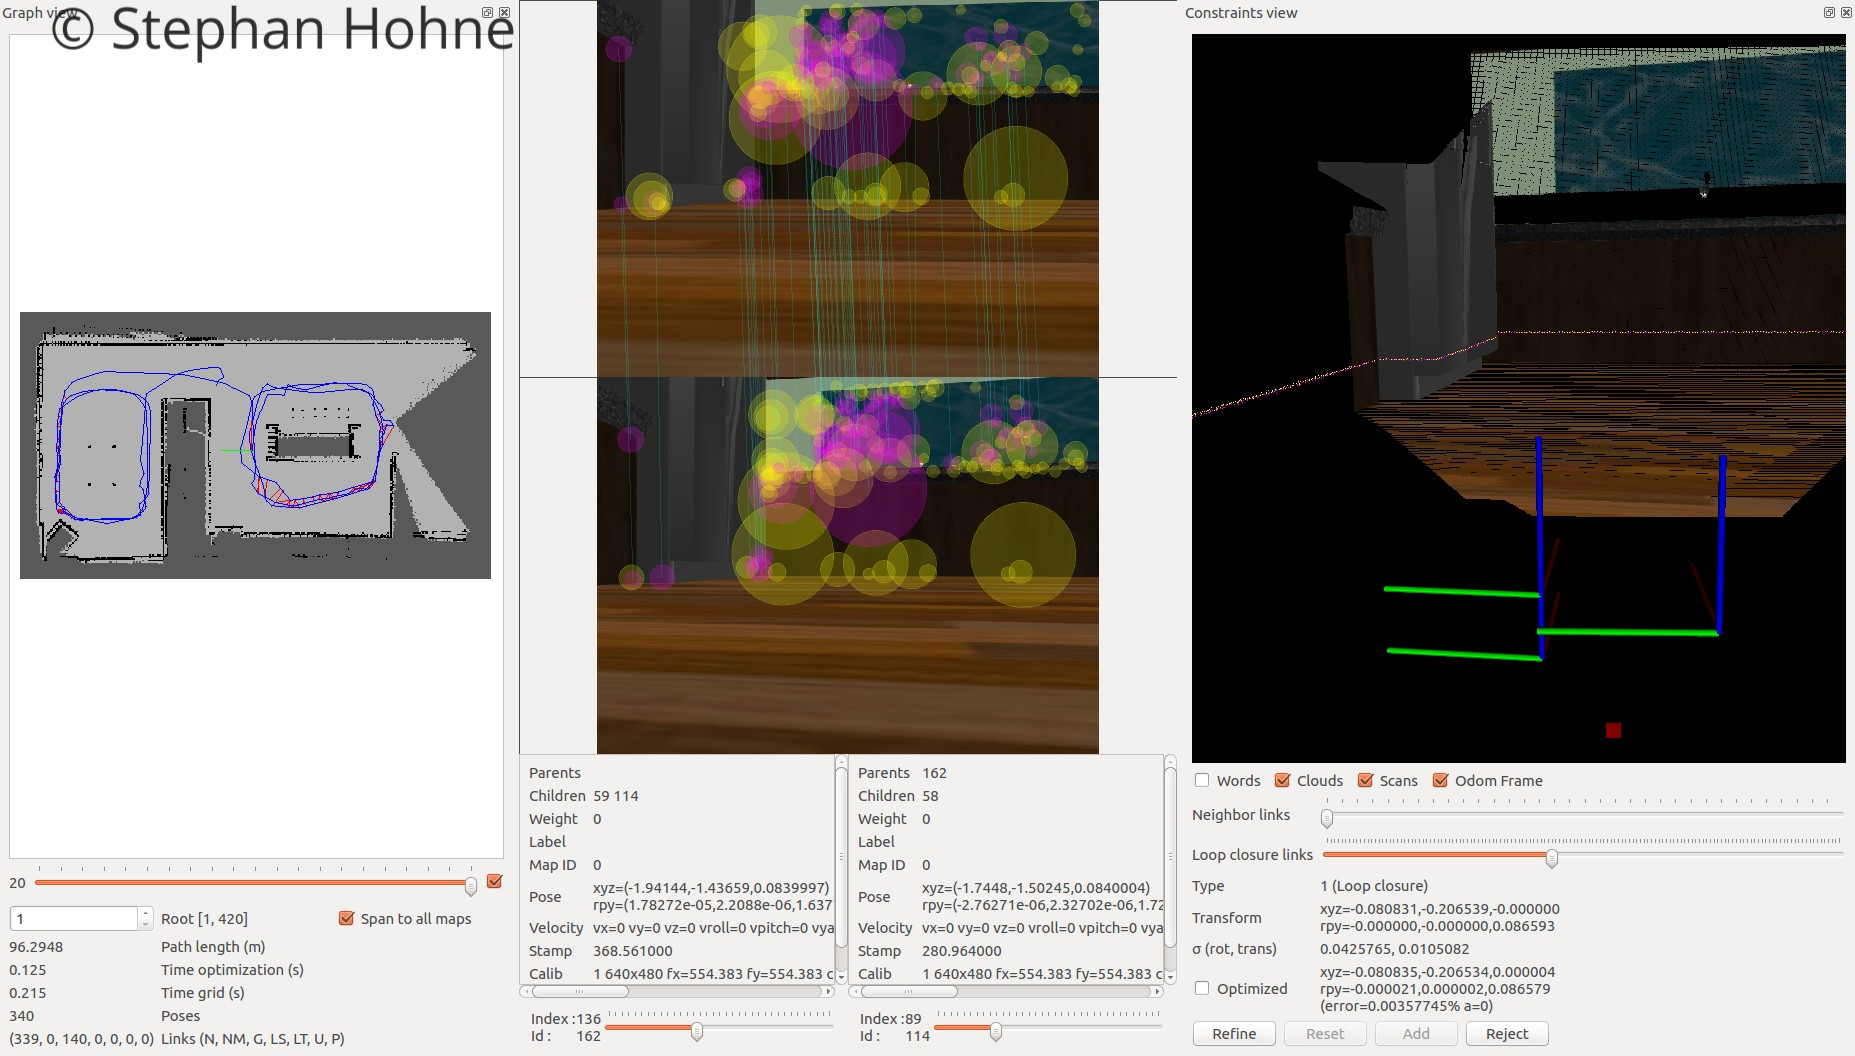
\includegraphics[width=\textwidth]{images/loop_closure_3.jpg}
      \caption{Loop closure in the map database \texttt{rtabmap\_kitchen\_dining\_run1.db}. Screenshot taken in \rtab\ Database Viewer.}
      \label{fig:loop_closure_3}
\end{figure*}
\begin{figure*}[thpb]
      \centering
      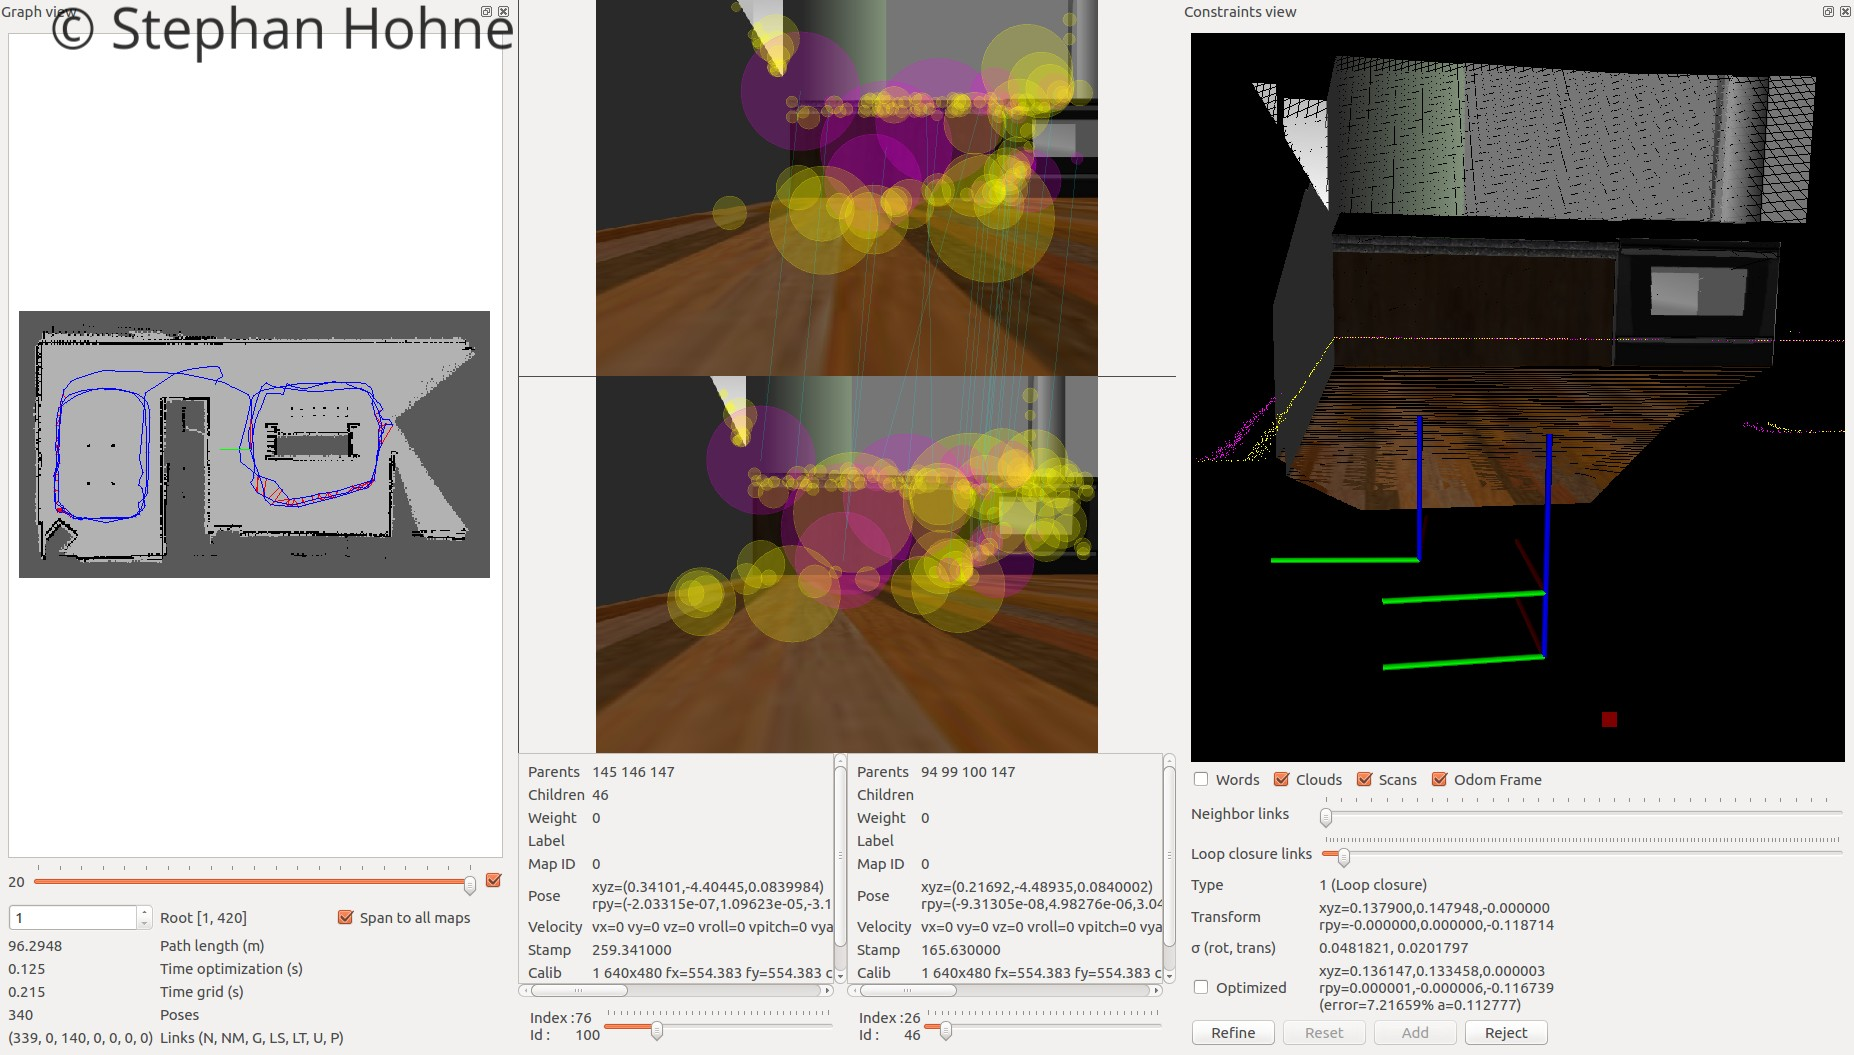
\includegraphics[width=\textwidth]{images/loop_closure_4.jpg}
      \caption{Loop closure in the map database \texttt{rtabmap\_kitchen\_dining\_run1.db}. Screenshot taken in \rtab\ Database Viewer.}
      \label{fig:loop_closure_4}
\end{figure*}

\begin{figure*}[thpb]
      \centering
      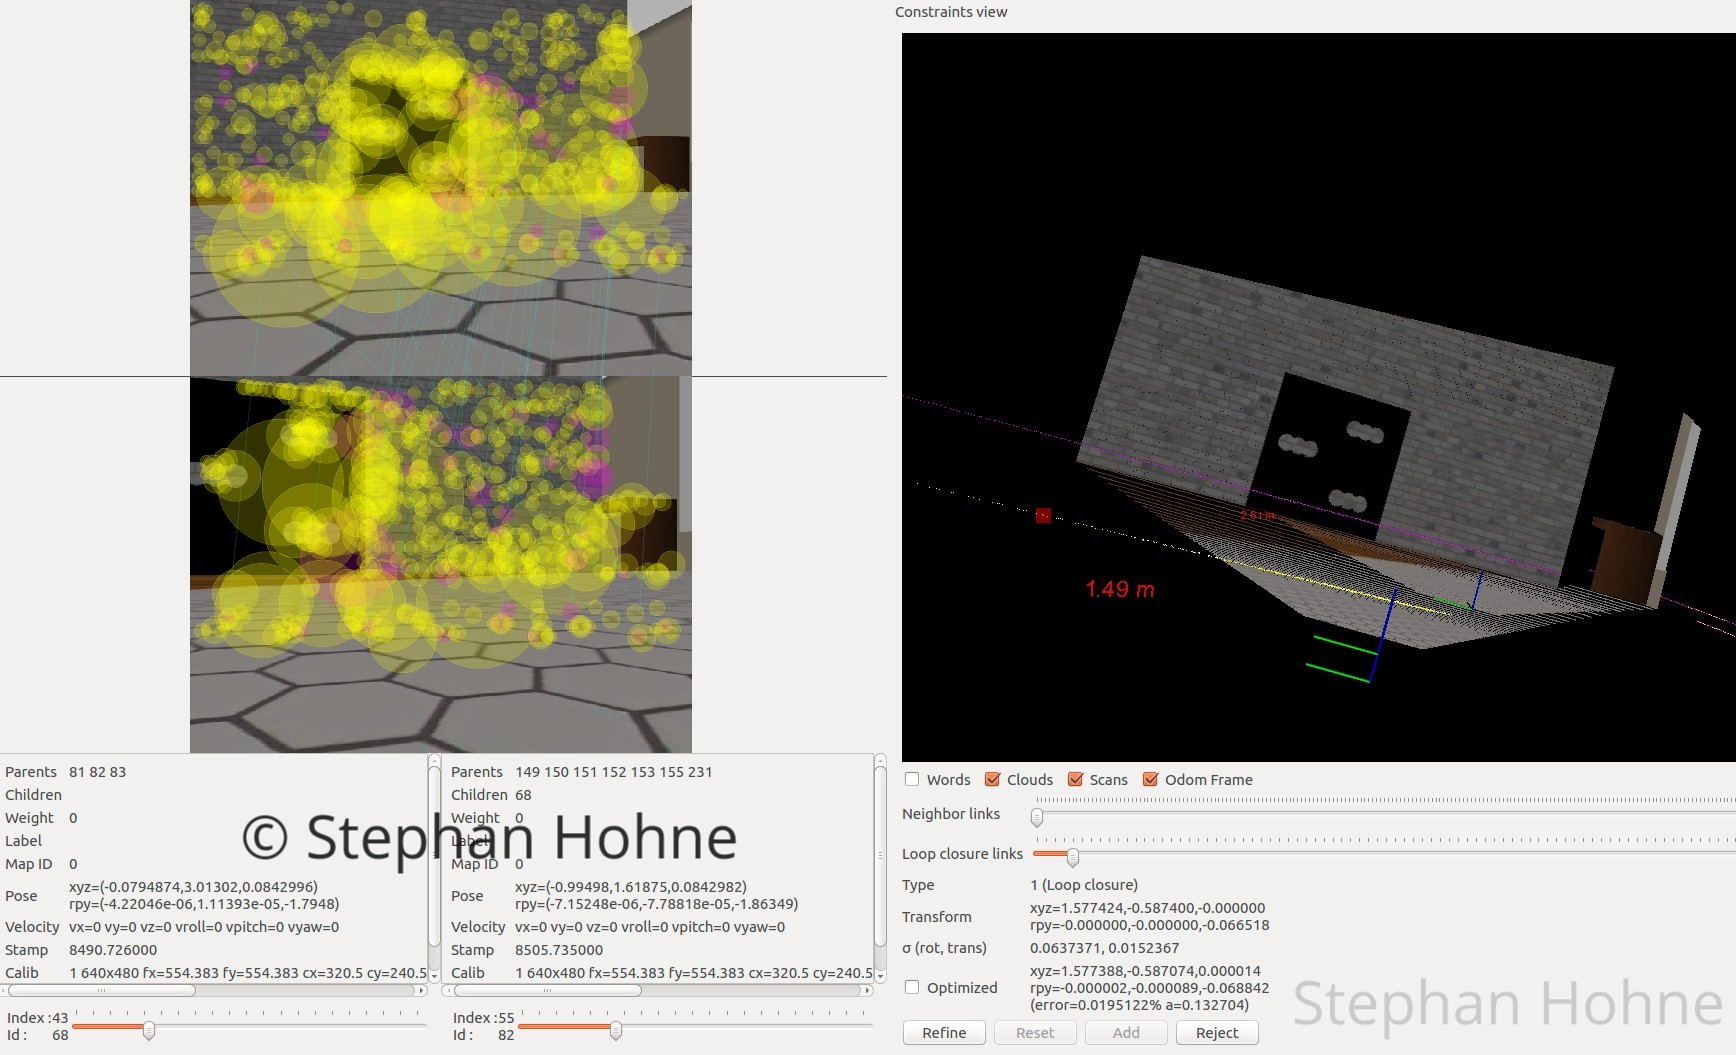
\includegraphics[width=\textwidth]{images/loop_closure_cafe.jpg}
      \caption{Example of a loop closure in the map database for the \texttt{cafe.world}. Screenshot taken in \rtab\ Database Viewer.}
      \label{fig:loop_closure_cafe}
\end{figure*}

\begin{figure*}[thpb]
      \centering
      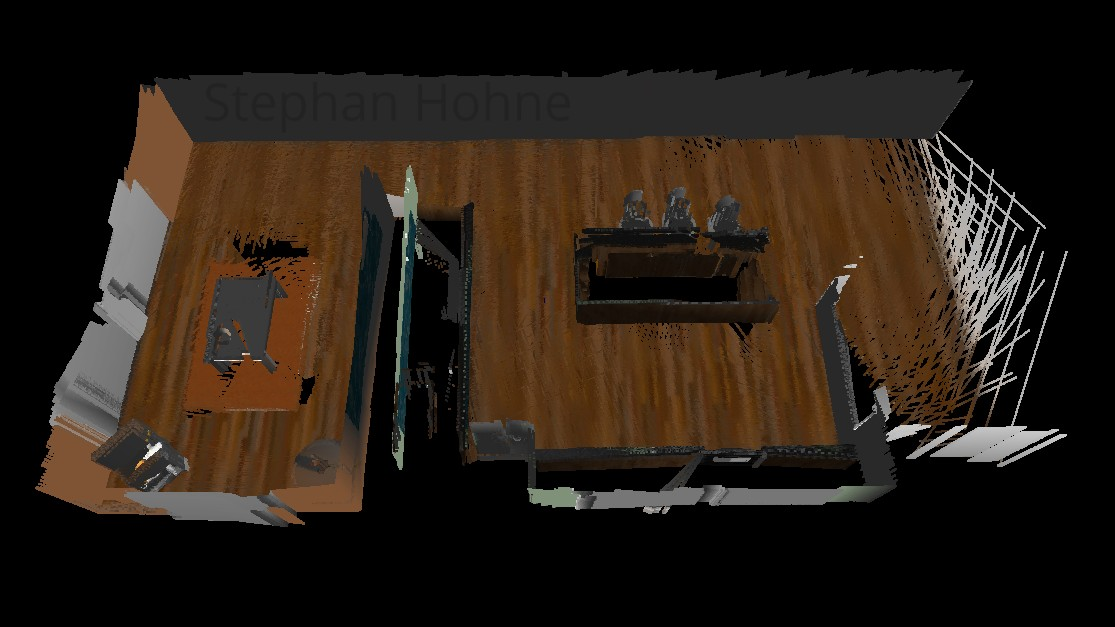
\includegraphics[width=\textwidth]{images/3D_point_cloud_kitchen_dining_settings_default.jpg}
      \caption{Reconstructed 3D point cloud of kitchen dining world. Default settings were used for reconstruction. Screenshot taken in \rtab\ Database Viewer.}
      \label{fig:3d_point_cloud_kitchen_dining_default}
\end{figure*}

\begin{figure*}[thpb]
      \centering
      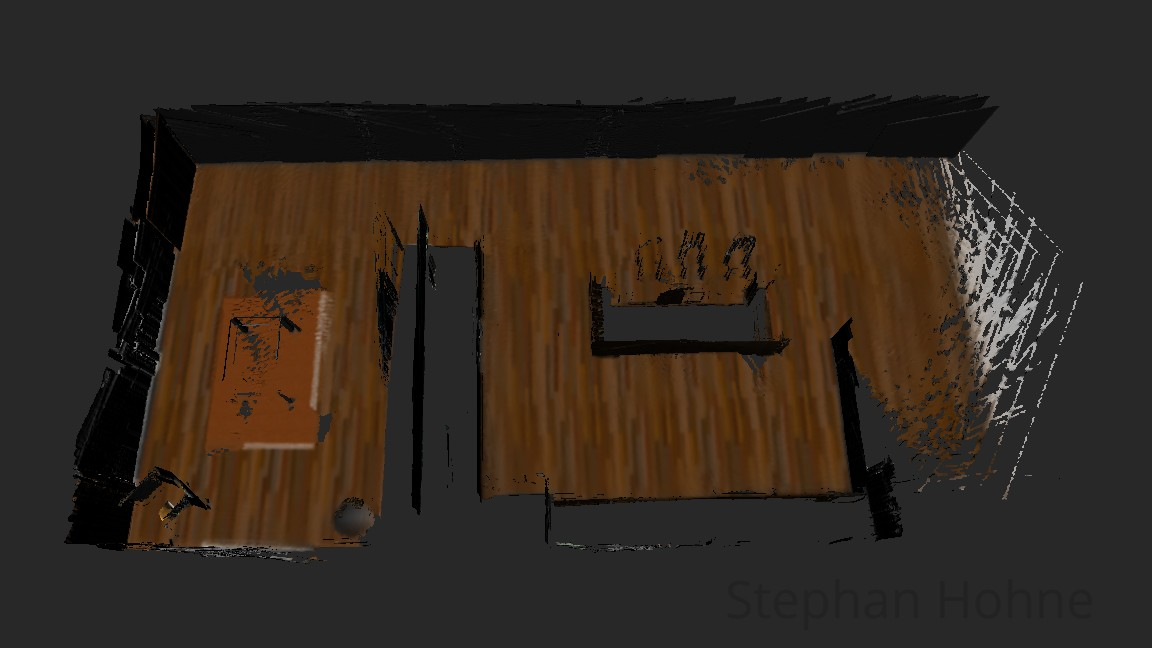
\includegraphics[width=\textwidth]{images/3D_point_cloud_kitchen_dining_settings_enhanced.jpg}
      \caption{Reconstructed 3D point cloud of kitchen dining world. Enhancement algorithms were applied for reconstruction. Screenshot taken in \rtab\ Database Viewer.}
      \label{fig:3d_point_cloud_kitchen_dining_enhanced}
\end{figure*}

\begin{figure*}[thpb]
      \centering
      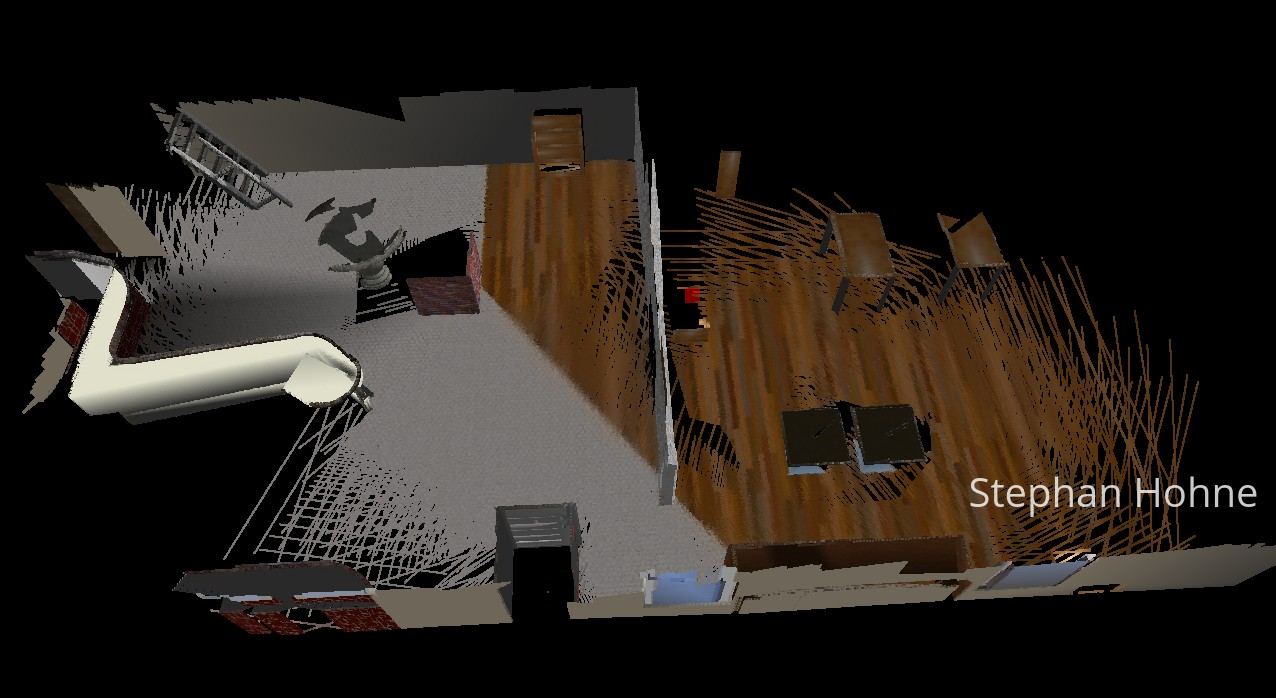
\includegraphics[width=\textwidth]{images/3D_cloud_cafe.jpg}
      \caption{Reconstructed 3D point cloud of cafe world. Default settings were used for reconstruction. Screenshot taken in \rtab\ Database Viewer.}
      \label{fig:cafe_3D_default}
\end{figure*}

\begin{figure*}[thpb]
      \centering
      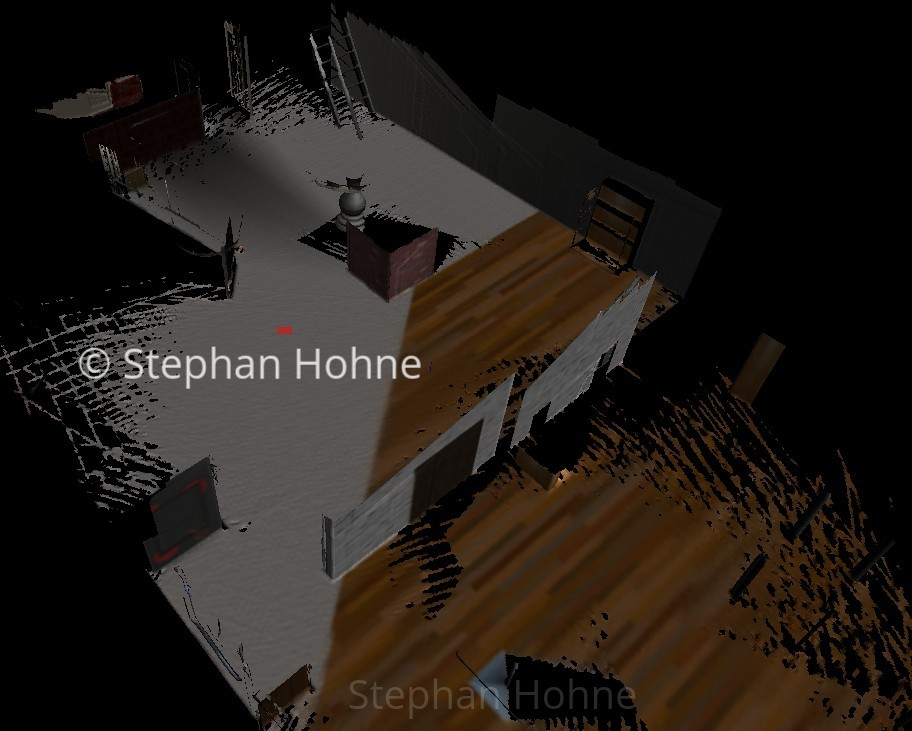
\includegraphics[width=\textwidth]{images/cafe_3D_left.jpg}
      \caption{3D view of the cafe world with enhanced reconstruction options enabled. Screenshot taken in \rtab\ Database Viewer.}
      \label{fig:cafe_3D_left}
\end{figure*}

\begin{figure*}[thpb]
      \centering
      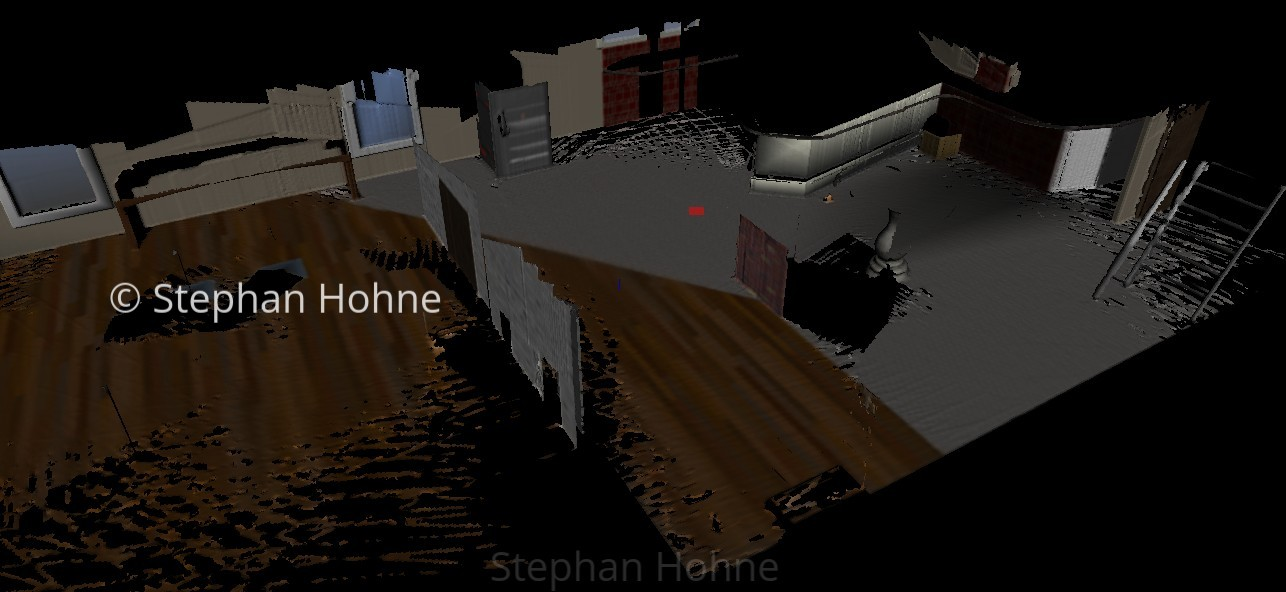
\includegraphics[width=\textwidth]{images/cafe_3D_right.jpg}
      \caption{3D view of the cafe world with enhanced reconstruction options enabled. Screenshot taken in \rtab\ Database Viewer.}
      \label{fig:cafe_3D_right}
\end{figure*}

\begin{figure*}[thpb]
      \centering
      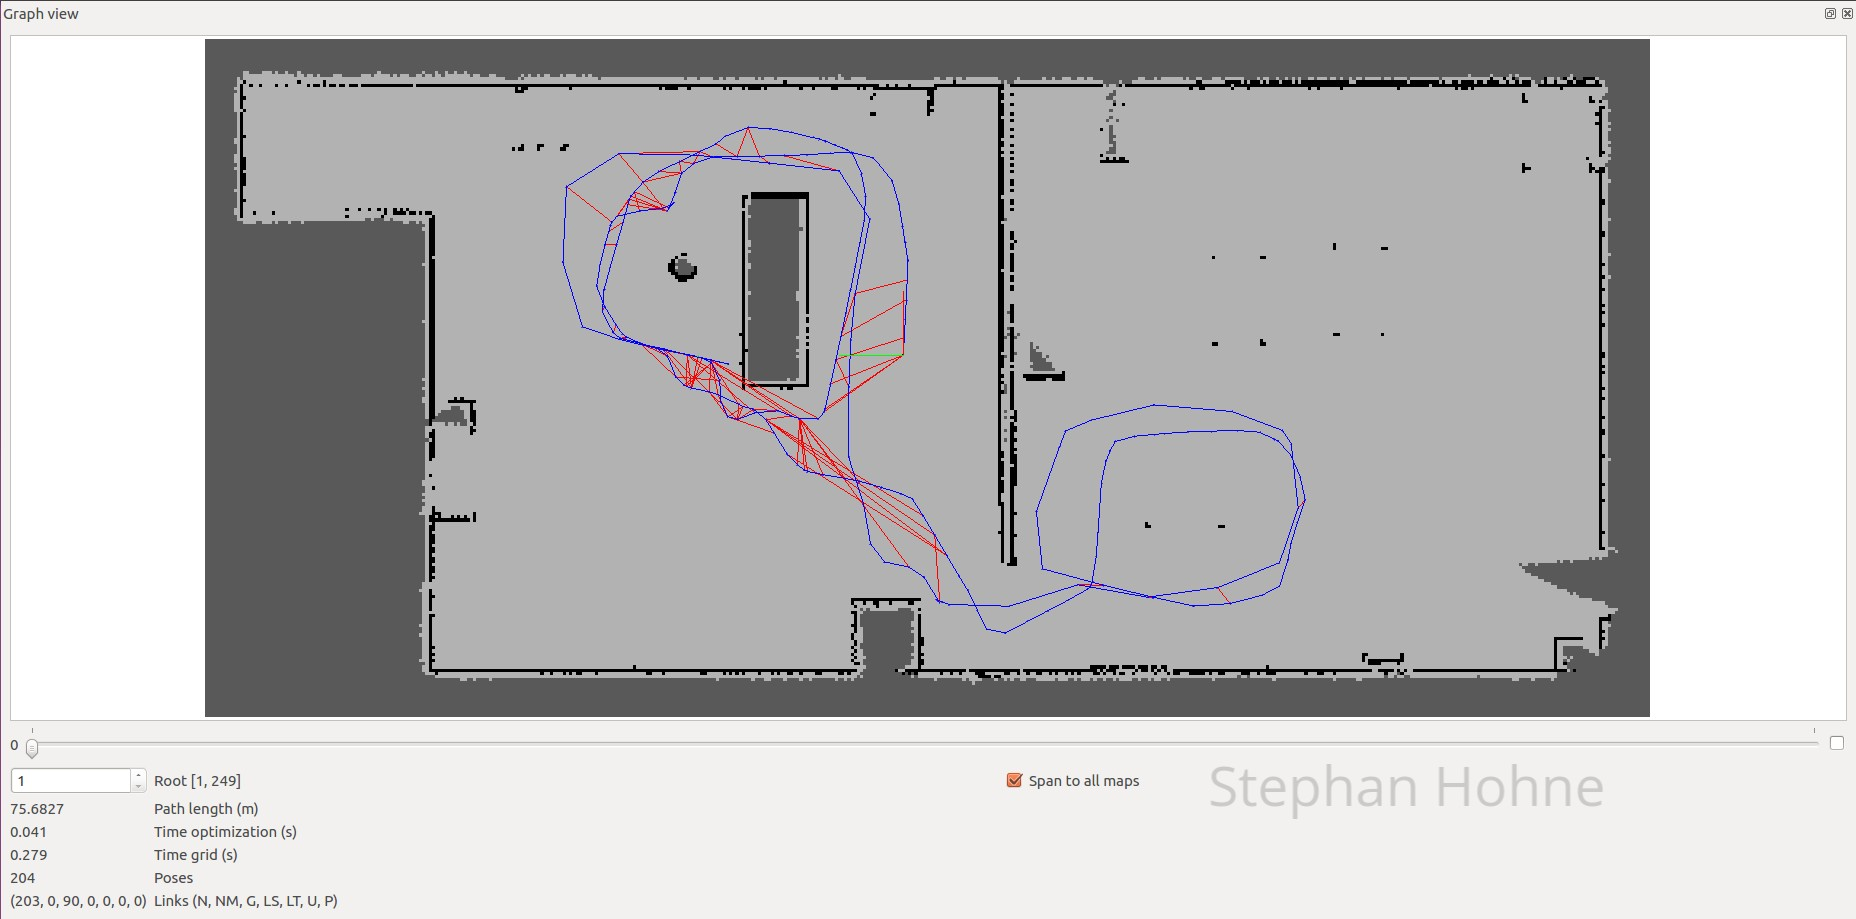
\includegraphics[width=\textwidth]{images/rtabmap_graph_view_cafe.jpg}
      \caption{Graph view showing the 2D map of the cafe world created during mapping run $2$. A total of $90$ global loop closures was detected. Screenshot taken in \rtab\ Database Viewer.}
      \label{fig:graph_view_cafe}
\end{figure*}

\bibliographystyle{ieeetr}
\begin{thebibliography}{6}

\bibitem{principles_of_robot_motion}
Howie Choset, Kevin M.\ Lynch, Seth Hutchinson, George Kantor, Wolfram Burgard, Lydia E.\ Kavraki and Sebastian Thrun, \textit{Principles of Robot Motion}, The MIT Press, 2005

\bibitem{probabilistic_robotics}
Sebastian Thrun, Wolfram Burgard and Dieter Fox, \textit{Probabilistic Robotics}, The MIT Press, 2005

\bibitem{hornung13auro}
Armin Hornung and Kai M. Wurm and Maren Bennewitz and Cyrill Stachniss and Wolfram Burgard, \textit{OctoMap: An Efficient Probabilistic 3D Mapping Framework Based on Octrees}, Autonomous Robots,2013, Software available at \href{http://octomap.github.com}{GitHub}

\bibitem{labbe14online}
Labbe, M. and Michaud, F., \textit{Online Global Loop Closure Detection for Large-Scale Multi-Session Graph-Based SLAM}, Proceedings of the IEEE/RSJ International Conference on Intelligent Robots and Systems, 2661-2666, Sept 2014

\bibitem{labbe13appearance}
Labbe, M. and Michaud, F., \textit{Appearance-Based Loop Closure Detection for Online Large-Scale and Long-Term Operation}, IEEE Transactions on Robotics Vol.\ 29 No.\ 3, 734-745, 2013

\bibitem{where_am_i}
Stephan Hohne, \textit{Robot Localization -- Where Am I?}, \href{https://github.com/S2H-Mobile/RoboND-Localization-Project}{project on GitHub}, 2018

\end{thebibliography}
\end{document}